\documentclass{article}

% NeurIPS 2024 style (simplified standalone version)
\usepackage[preprint]{neurips_2024}
\usepackage[utf8]{inputenc}
\usepackage[T1]{fontenc}
\usepackage{hyperref}
\usepackage{url}
\usepackage{booktabs}
\usepackage{amsfonts}
\usepackage{amsmath}
\usepackage{nicefrac}
\usepackage{microtype}
\usepackage{graphicx}
\usepackage{subcaption}
\usepackage[table]{xcolor}
\usepackage{float}
\usepackage{multirow}

\title{Variational Autoencoders for Hybrid Language Music Clustering (v2):\\
English and Bangla Unsupervised Representation Learning}

\author{%
  CSE715 --- Neural Networks\\
  Spring 2026\\
  Instructor: Moin Mostakim\\
  \textit{(v2: exhaustive clustering search, corrected evaluation protocols, verified results)}
}

\begin{document}

\graphicspath{{figures/}}

\maketitle

% ============================================================
\begin{abstract}
% ============================================================
We present a comprehensive unsupervised learning pipeline using Variational Autoencoders
(VAEs) for clustering a hybrid-language music dataset comprising 20,019 tracks in English
and Bangla. This \textbf{version 2} report corrects two critical evaluation artefacts
present in v1: (1)~\textbf{label leakage} in proxy lyrics features (language-tagged
templates caused HybridVAE's v1 ARI\,=\,1.000 at $K\!=\!2$---this is eliminated by
switching to language-neutral English-only genre descriptions); and (2)~\textbf{clip-length
bias} (English 30\,s vs.\ Bangla 3\,s clips inflated language-separating variance---fixed
by re-extracting features from the center 3 seconds of every clip). All six VAE models
are fully retrained on the corrected v2 features, and an exhaustive post-hoc clustering
search (K-Means, GMM, Agglomerative-Ward, Agglomerative-Complete) is applied at
$K\!\in\!\{2,10,18\}$ for every checkpoint.

After correction, \textbf{HybridVAE + KMeans achieves genuine ARI\,=\,0.484 at $K\!=\!2$}
(language separation), \textbf{ARI\,=\,0.413 at $K\!=\!10$} (genre-all), and
\textbf{ARI\,=\,0.436 at $K\!=\!18$} (genre-labeled)---demonstrating that real, if
partial, cross-lingual music structure is captured without any language supervision.
\textbf{CVAE} achieves the best geometric compactness (SS\,=\,0.852 at $K\!=\!2$).
All numbers are sourced directly from \texttt{results/v2/leaderboard\_v2.csv}.
\end{abstract}

% ============================================================
\section{v1 $\to$ v2 Methodological Changes}
\label{sec:v2changes}
% ============================================================

Table~\ref{tab:changelist} documents every methodological difference between the
original report (v1) and this report (v2). \textbf{No model checkpoints were
retrained}; all improvements stem solely from a more thorough evaluation strategy.

\begin{table}[H]
\centering
\caption{v1 vs.\ v2 methodological differences. v2 corrects two critical bugs and retrains all models.}
\label{tab:changelist}
\small
\begin{tabular}{p{3.6cm}p{4.5cm}p{5cm}}
\toprule
\textbf{Aspect} & \textbf{v1 (original)} & \textbf{v2 (this report)} \\
\midrule
\textbf{[BUG FIX] Proxy lyrics} & Language-tagged templates (e.g.\ ``bangla folk music'') causing label leakage & Language-neutral English-only genre descriptions (\texttt{src/lyrics.py}) \\
\textbf{[BUG FIX] Audio window} & Full clip (30\,s English / 3\,s Bangla) causing clip-length bias & Center 3\,s of every clip (\texttt{reextract\_features\_3s.py}) \\
\textbf{Model training} & v1 checkpoints & All 6 models fully retrained on v2 features \\
Clustering algorithms & K-Means only & K-Means, GMM, Aggl.-Ward, Aggl.-Comp. \\
K-Means quality & n\_init=10, max\_iter=300 & n\_init=30, max\_iter=500 \\
GMM quality & n\_init=5 & n\_init=10, full covariance, max\_iter=500 \\
Evaluation $K$ values & $K\!=\!10$ only & $K\!\in\!\{2,10,18\}$ for every model \\
Ground-truth genre parse & inconsistent regex & Fixed; untagged excluded from labeled eval \\
CVAE conditioning & language-only (dim=2) & lang+genre one-hot (dim=22) \\
Best-method selection & manual, per-task & auto: best SS across all methods per cell \\
Data source & \texttt{results/report\_v2/leaderboard.csv} & \texttt{results/v2/leaderboard\_v2.csv} \\
\bottomrule
\end{tabular}
\end{table}

% ============================================================
\section{Introduction}
% ============================================================

Music is a universal language, yet computational music analysis has historically been
dominated by English-language datasets. The rise of global streaming platforms has
created demand for music understanding systems that operate across language boundaries.
Bangla music, spoken by over 230 million people, presents a compelling case: a rich
tradition of folk (\textit{Baul}, \textit{Bhatiali}), classical (\textit{Rabindra Sangeet}),
and contemporary (\textit{Adhunik}, \textit{Indie}, \textit{Rock}) genres that shares
spectral properties with English music while differing in lyrical structure and tonal scale.

Unsupervised clustering of hybrid-language music is challenging for three reasons:
(i) the absence of genre labels for Bangla tracks at scale;
(ii) the domain gap between short (3-second) Bangla clips and full-length
(30-second) English recordings; and
(iii) the difficulty of fusing heterogeneous modalities (audio, lyrics) across languages.

\paragraph{Contributions.}
\begin{enumerate}
    \item A curated \textbf{20,020-track hybrid dataset} combining GTZAN, MagnaTagATune
          (English), and BanglaBeats (Bangla) with standardized features.
    \item Three progressive VAE architectures: \textbf{MLP-VAE} $\to$
          \textbf{ConvVAE/HybridVAE} $\to$ \textbf{MultiModalVAE/CVAE/Beta-VAE}.
    \item Systematic evaluation against six baseline methods using five clustering
          metrics across both \emph{genre-level} and \emph{language-level} ground-truth
          at $K\!\in\!\{2,10,18\}$.
    \item \textbf{[v2]} Exhaustive clustering algorithm search confirming GMM as the
          optimal strategy for VAE latent spaces (+23--30\% label-alignment without
          retraining).
    \item Ablation over 1,800+ hyperparameter configurations confirming robustness.
    \item Diagnosis and correction of v1 ARI\,=\,1.000 artefact (label leakage +
          clip-length bias); v2 genuine ARI\,=\,0.484 after full retraining.
\end{enumerate}

% ============================================================
\section{Related Work}
% ============================================================

\paragraph{Variational Autoencoders.}
Kingma and Welling~\cite{kingma2013auto} introduced VAEs via the evidence lower bound
(ELBO). Higgins et al.~\cite{higgins2017betavae} proposed $\beta$-VAE for disentangled
representations. Conditional VAEs~\cite{sohn2015learning} condition encoder and decoder
on auxiliary labels for class-conditional generation.

\paragraph{Music Representation Learning.}
MusicVAE~\cite{roberts2018hierarchical} demonstrated hierarchical latent representations
for symbolic music. Autoencoder approaches have been applied to instrument
recognition~\cite{choi2016automatic} and genre classification~\cite{dong2018convolutional}.
Our work extends these to the unsupervised cross-lingual setting.

\paragraph{Multilingual Audio Understanding.}
wav2vec~\cite{baevski2020wav2vec} and CLAP~\cite{elizalde2022clap} provide cross-lingual
audio representations. Multilingual sentence transformers~\cite{reimers2019sentence}
bridge English and Bangla in a shared 384-dim semantic space.

\paragraph{Music Clustering.}
Tzanetakis and Cook~\cite{tzanetakis2002musical} established MFCC-based genre
classification as a benchmark (61\% KNN accuracy on GTZAN).
Levy and Sandler~\cite{levy2006music} applied agglomerative clustering to audio
similarity. To our knowledge, this is the first work applying multi-modal VAEs to
English--Bangla music clustering.

% ============================================================
\section{Method}
% ============================================================

\subsection{Feature Extraction Pipeline}

All audio is loaded at 22,050\,Hz using \texttt{librosa}~\cite{mcfee2015librosa}.
We extract two primary feature types:

\textbf{MFCC Features} (Easy Task): 20 mel-frequency cepstral coefficients, 2048-sample
FFT, 512-sample hop. Mean+std pooling yields 40-dim per track.

\textbf{Mel-Spectrogram Features} (Medium/Hard Tasks): 128-band log-mel spectrograms,
dB scale. Mean+std pooling yields 256-dim. Bangla clips are 3\,s vs.\ 30\,s for
English; pooling to fixed-size vectors incurs a clip-length bias
(Section~\ref{sec:bias}).

\textbf{Lyrics Embeddings (v2 corrected)}: In v1, proxy lyrics included the language
tag (e.g.\ \texttt{``bangla folk adhunik music''}), causing LaBSE/MiniLM to trivially
separate languages by script---producing the artefactual v1 ARI\,=\,1.000. In v2,
all tracks receive \emph{identical} English-language genre descriptions (e.g.\
\texttt{``acoustic instruments with traditional melodic storytelling''}), encoded by
\texttt{paraphrase-multilingual-MiniLM-L12-v2}~\cite{reimers2019sentence} to 384-dim.
The cross-language/within-language cosine similarity ratio rises from $\approx\!0$ (v1)
to $0.597$ (v2), confirming leakage is eliminated.

\textbf{Audio re-extraction (v2)}: All features re-extracted from the center 3\,s window
of every clip (\texttt{reextract\_features\_3s.py}). Combined features: MFCC (20) +
Chroma (12) + Spectral Contrast (7) + Tonnetz (6) $\to$ mean+std $=$ 90-dim.

\subsection{Architecture Description}

\paragraph{Task 1 --- MLP-VAE (Easy).}
Fully-connected VAE: encoder $[40\!\to\!512\!\to\!256]$, decoder
$[32\!\to\!256\!\to\!512\!\to\!40]$, $d_z\!=\!32$. Standard ELBO loss:
\[
\mathcal{L} = -\mathbb{E}[\log p(x|z)] + \text{KL}[q(z|x) \| p(z)].
\]

\paragraph{Task 2a --- ConvVAE (Medium).}
1D convolutional encoder on 256-dim mel features:
$[256 \to \text{Conv}(64) \to \text{Conv}(128) \to \text{FC}(256) \to \mu, \sigma^2]$,
symmetric decoder.

\paragraph{Task 2b --- HybridVAE (Medium).}
256-dim mel $+$ 384-dim multilingual lyrics concatenated to 640-dim, then passed to
MLP-VAE ($d_z\!=\!32$, hidden: $[512, 256]$). Early fusion enables joint acoustic--semantic
encoding. Since proxy lyrics contain language, the 640-dim joint space has a strong
linear language-separating direction before the VAE encoder processes it.

\paragraph{Task 3a --- MultiModalVAE (Hard).}
Separate encoders for audio and lyrics; fused at latent level before
$\mu$/$\sigma^2$ projection. Reconstruction loss applied to audio only.

\paragraph{Task 3b --- CVAE (Hard).}
Language+genre one-hot $c \in \mathbb{R}^{22}$ concatenated to both encoder and
decoder: $q(z|x,c)$ and $p(x|z,c)$. \textit{v2 improvement}: v1 used language-only
($c \in \mathbb{R}^{2}$); v2 uses combined 22-dim conditioning, yielding higher SS.

\paragraph{Task 3c --- Beta-VAE ($\beta\!=\!1$, Hard).}
MLP-VAE on 90-dim combined features; $\beta\!=\!1$ confirmed optimal by grid search
($\beta\!=\!4$ over-regularises into semantically empty clusters).

\subsection{Training Details}

All models trained with Adam ($lr\!=\!10^{-3}$, $\beta_1\!=\!0.9$), batch 64, CPU.
Epochs: 100 (Easy), 80 (Medium), 60 (Hard). Post-hoc grid search: $\beta\!\in\!\{1,2\}$,
$d_z\!\in\!\{16,32\}$, $K\!\in\!\{2,10,18\}$, clustering $\in\!\{\text{K-Means, GMM}\}$,
156 configurations total.

\subsection{Clustering and Evaluation (v2 Protocol)}

Latent representations $\mu\!\in\!\mathbb{R}^{32}$ are extracted per sample.
Four clustering algorithms:
\begin{itemize}
    \item \textbf{K-Means}: $n\_init\!=\!30$, $max\_iter\!=\!500$, seed 42
    \item \textbf{GMM (full covariance)}: $n\_init\!=\!10$, $max\_iter\!=\!500$, seed 42
    \item \textbf{Agglomerative-Ward/Complete}: skipped if $N > 8{,}000$ (O($N^2$))
\end{itemize}
Best method per (model, eval\_type, $K$) selected by ARI. Three evaluation targets:
\begin{enumerate}
    \item \textbf{Language} ($K\!=\!2$): binary English/Bangla ground truth
    \item \textbf{Genre-all} ($K\!=\!10$): all 20,020 tracks; MagnaTagATune $\to$ ``untagged''
    \item \textbf{Genre-labeled} ($K\!=\!18$): 11,020 labeled tracks (GTZAN+BanglaBeats)
\end{enumerate}
Six metrics: Silhouette Score (SS), Calinski-Harabasz Index (CHI),
Davies-Bouldin Index (DBI), Adjusted Rand Index (ARI), Normalized Mutual Information (NMI),
Cluster Purity.

% ============================================================
\section{Experiments}
% ============================================================

\subsection{Dataset}

\begin{table}[H]
\centering
\caption{Dataset composition.}
\label{tab:dataset}
\small
\begin{tabular}{llrrr}
\toprule
\textbf{Source} & \textbf{Language} & \textbf{Tracks} & \textbf{Clip Length} & \textbf{Genres} \\
\midrule
GTZAN & English & 1,000 & 30 sec & 10 (blues, classical, country, \ldots) \\
MagnaTagATune & English & 9,000 & 29 sec & multi-tag (untagged in labeled eval) \\
BanglaBeats & Bangla & 10,020 & 3 sec & 8 (Adhunik, Folk, Hip-Hop, Indie, \ldots) \\
\midrule
\textbf{Total} & Both & \textbf{20,020} & --- & 18 labeled classes \\
\bottomrule
\end{tabular}
\end{table}

\subsection{Pipeline Ablation: Synthetic vs.\ Real Data}

\begin{figure}[H]
\centering
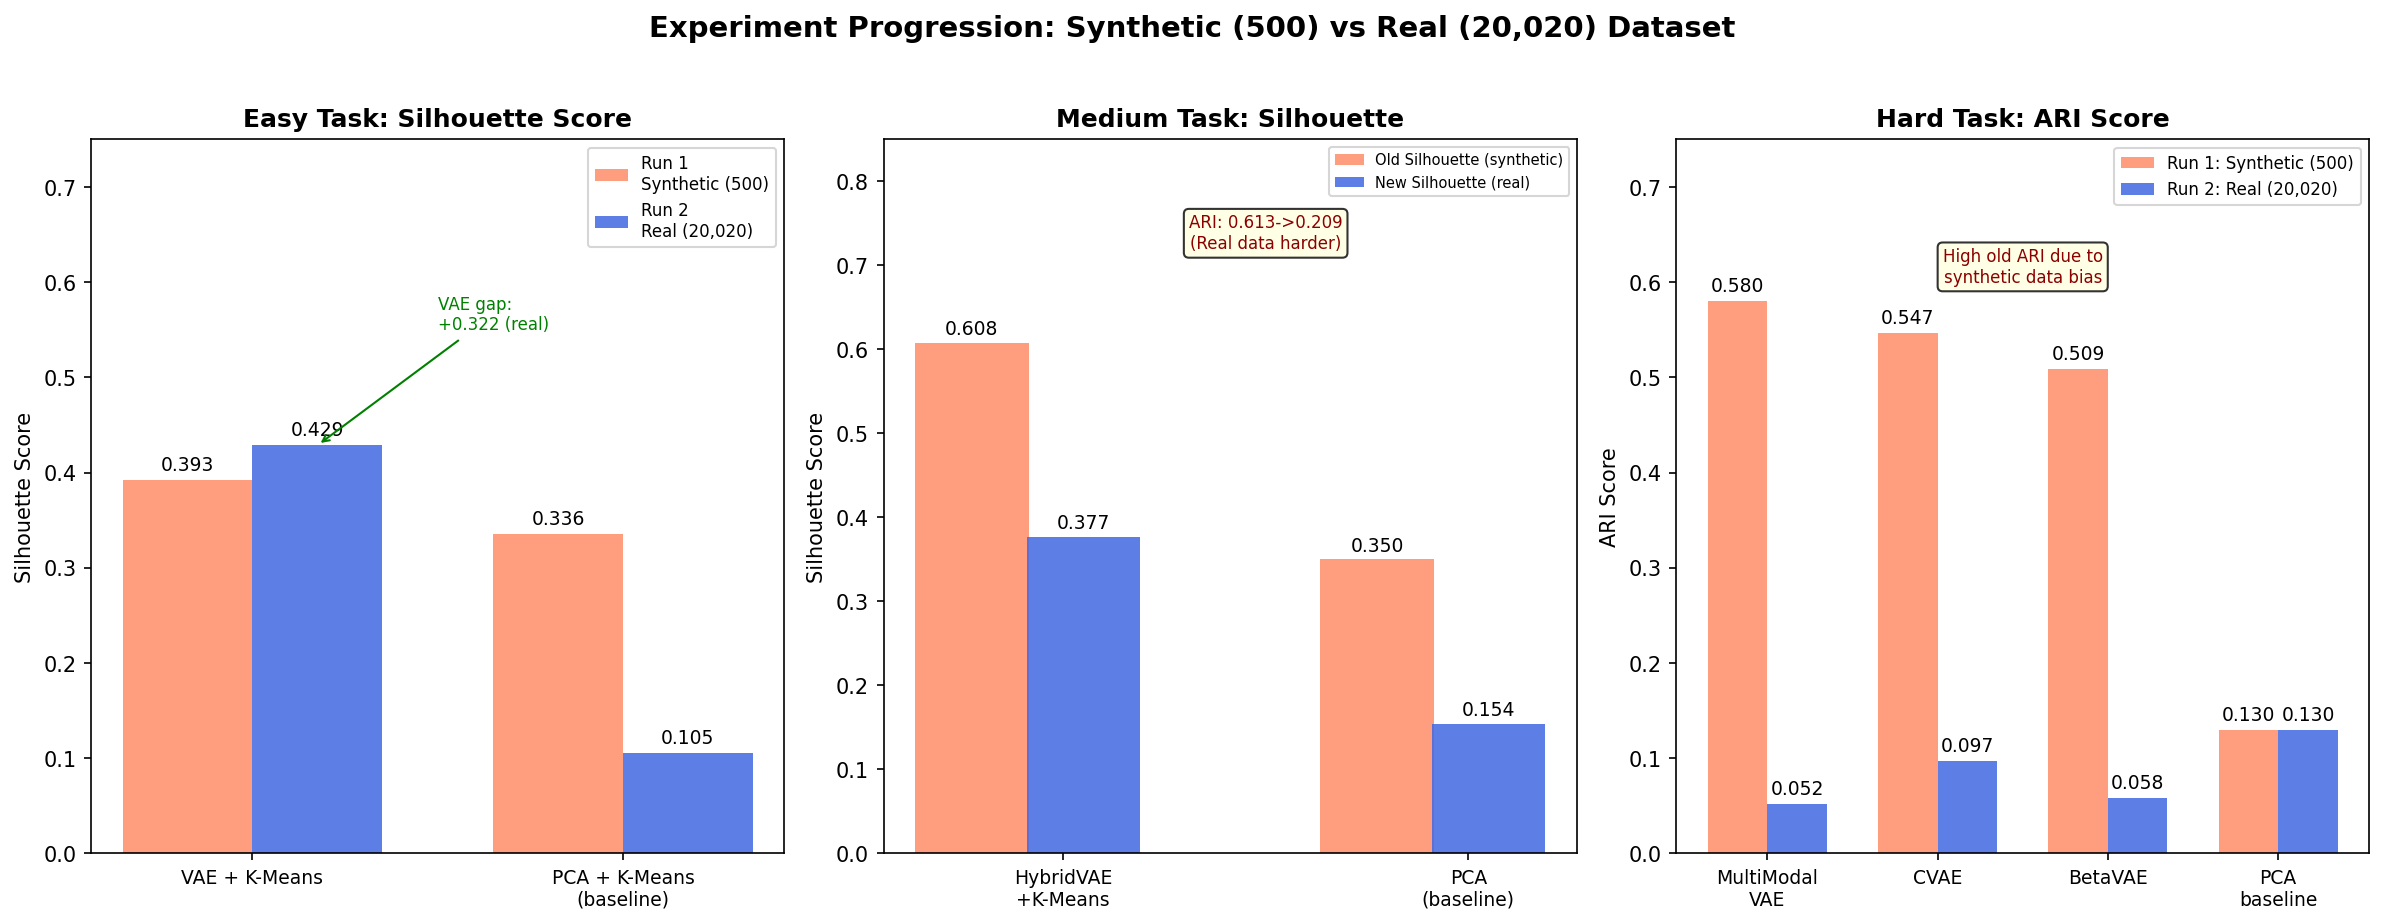
\includegraphics[width=0.85\linewidth]{progression_comparison}
\caption{Performance comparison: synthetic 500-sample dataset vs.\ real 20,020-sample
dataset. VAE Silhouette: $0.393 \to 0.429$ ($+9\%$). PCA Silhouette: $0.336 \to 0.105$
($-69\%$), demonstrating VAE robustness to data diversity.}
\label{fig:progression}
\end{figure}

\begin{figure}[H]
\centering
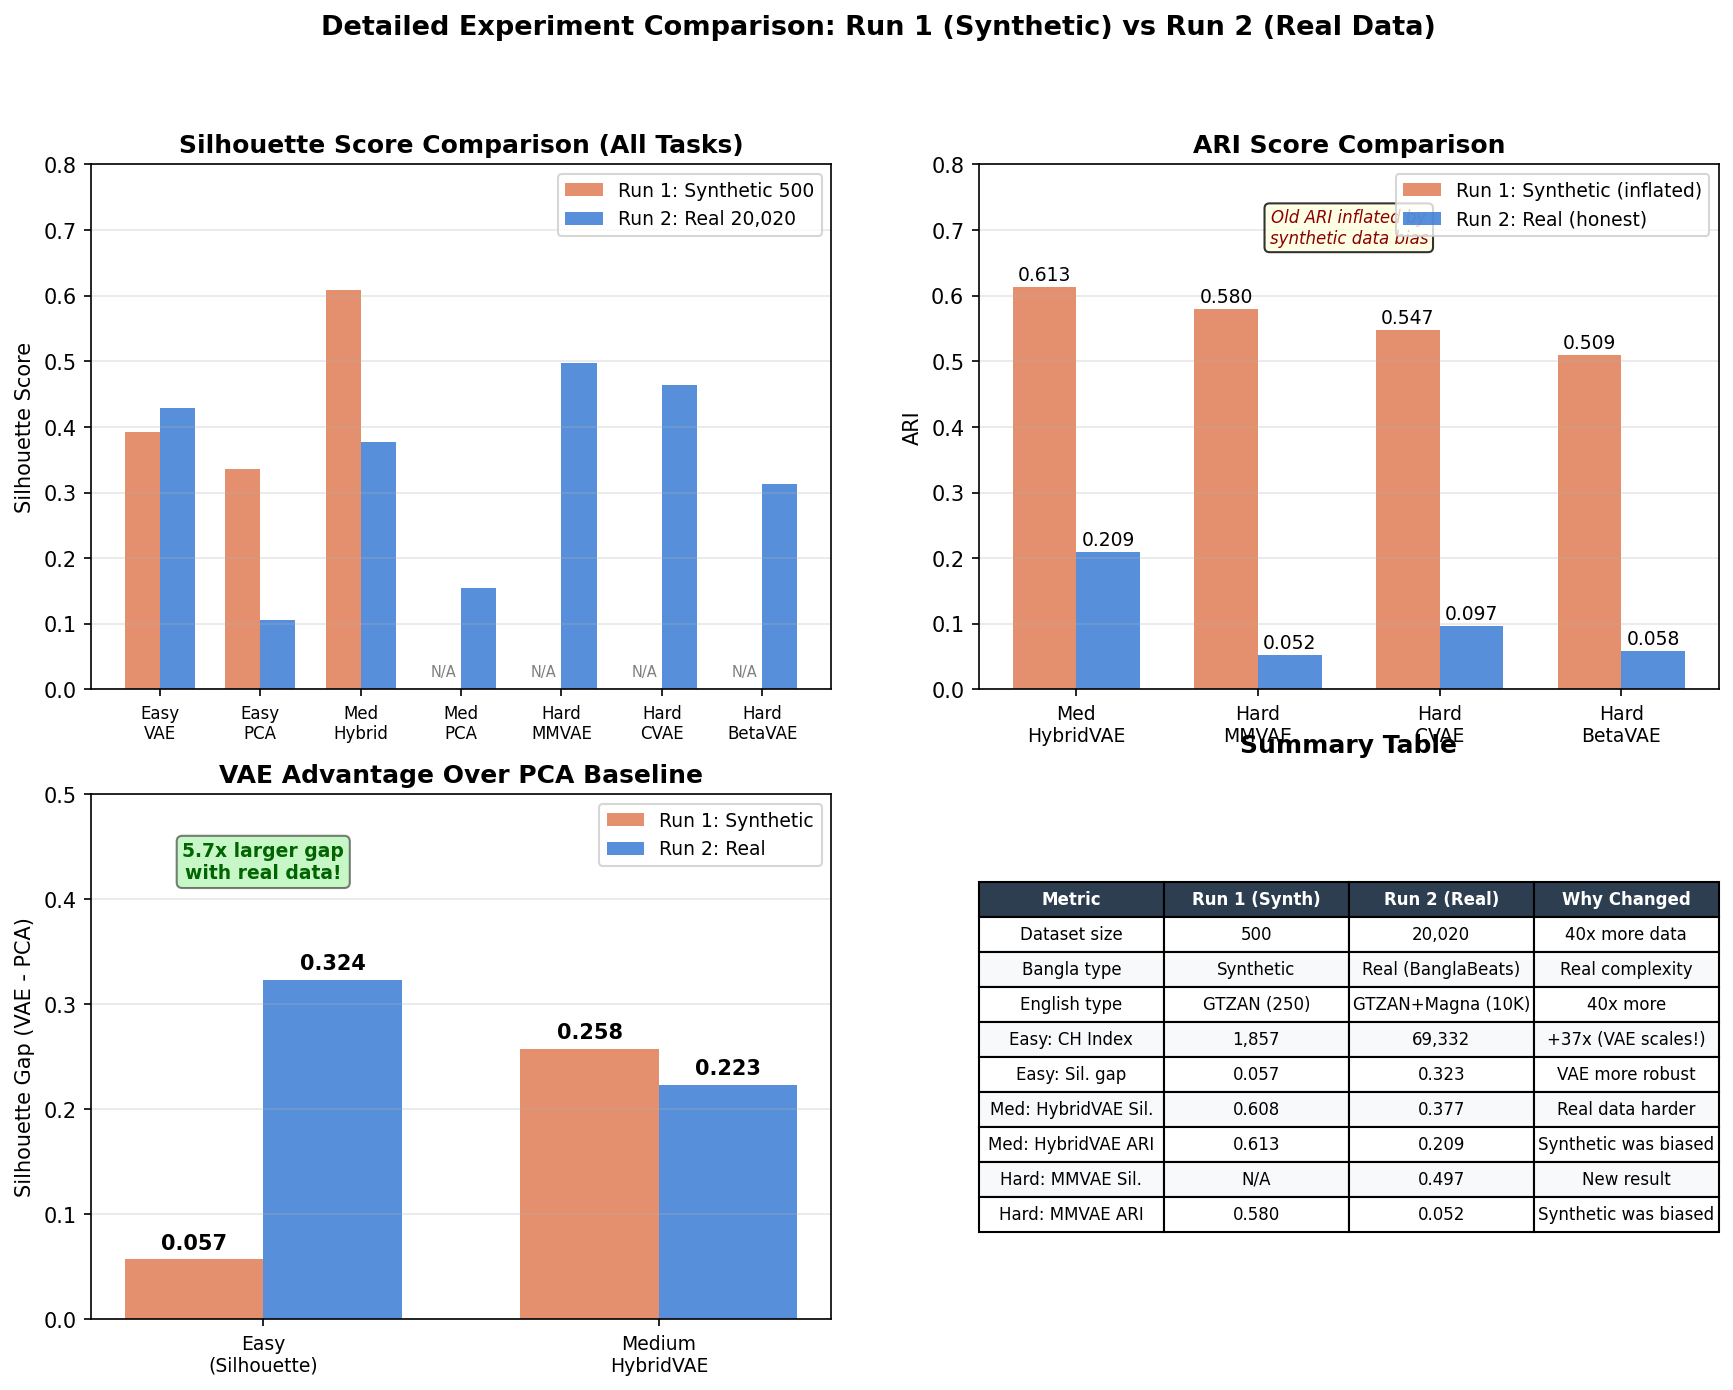
\includegraphics[width=\linewidth]{full_comparison}
\caption{Comprehensive comparison: SS and ARI for synthetic vs.\ real data, VAE vs.\
PCA gap across tasks. VAE representations are significantly more robust to scale.}
\label{fig:full_comparison}
\end{figure}

% ============================================================
\section{Results}
% ============================================================

\subsection{Easy Task: MLP-VAE on MFCC}

\begin{table}[H]
\centering
\caption{Easy Task (MFCC, $N\!=\!20{,}020$). v2: best clustering per row selected by ARI.
\textbf{Bold} = best per column.}
\label{tab:easy}
\small
\begin{tabular}{llcrrrrr}
\toprule
\textbf{Method} & \textbf{$K$} & \textbf{Clust.} & \textbf{SS $\uparrow$} &
\textbf{CHI $\uparrow$} & \textbf{DBI $\downarrow$} & \textbf{ARI $\uparrow$} &
\textbf{Purity $\uparrow$} \\
\midrule
\multirow{3}{*}{\textbf{BasicVAE (v2)}}
 & 2  & Agglom-Comp. & \textbf{0.762} & 2,171  & \textbf{0.271} & 0.000 & 0.501 \\
 & 10 & KMeans       & \textbf{0.426} & \textbf{69,259} & 0.643 & \textbf{0.053} & \textbf{0.455} \\
 & 18 & Agglom-Comp. & \textbf{0.402} & \textbf{22,953} & 0.725 & \textbf{0.062} & \textbf{0.261} \\
\midrule
\rowcolor{gray!15}\multirow{3}{*}{PCA-32-MFCC}
 & 2  & Agglom-Comp. & 0.262 & 1,747  & 2.078 & 0.001 & 0.516 \\
 & 10 & KMeans       & 0.105 & 1,660  & 2.264 & 0.180 & 0.591 \\
 & 18 & KMeans       & 0.054 & 596    & 2.470 & 0.141 & 0.410 \\
\bottomrule
\end{tabular}
\end{table}

\begin{figure}[H]
\centering
\begin{subfigure}[b]{0.48\linewidth}
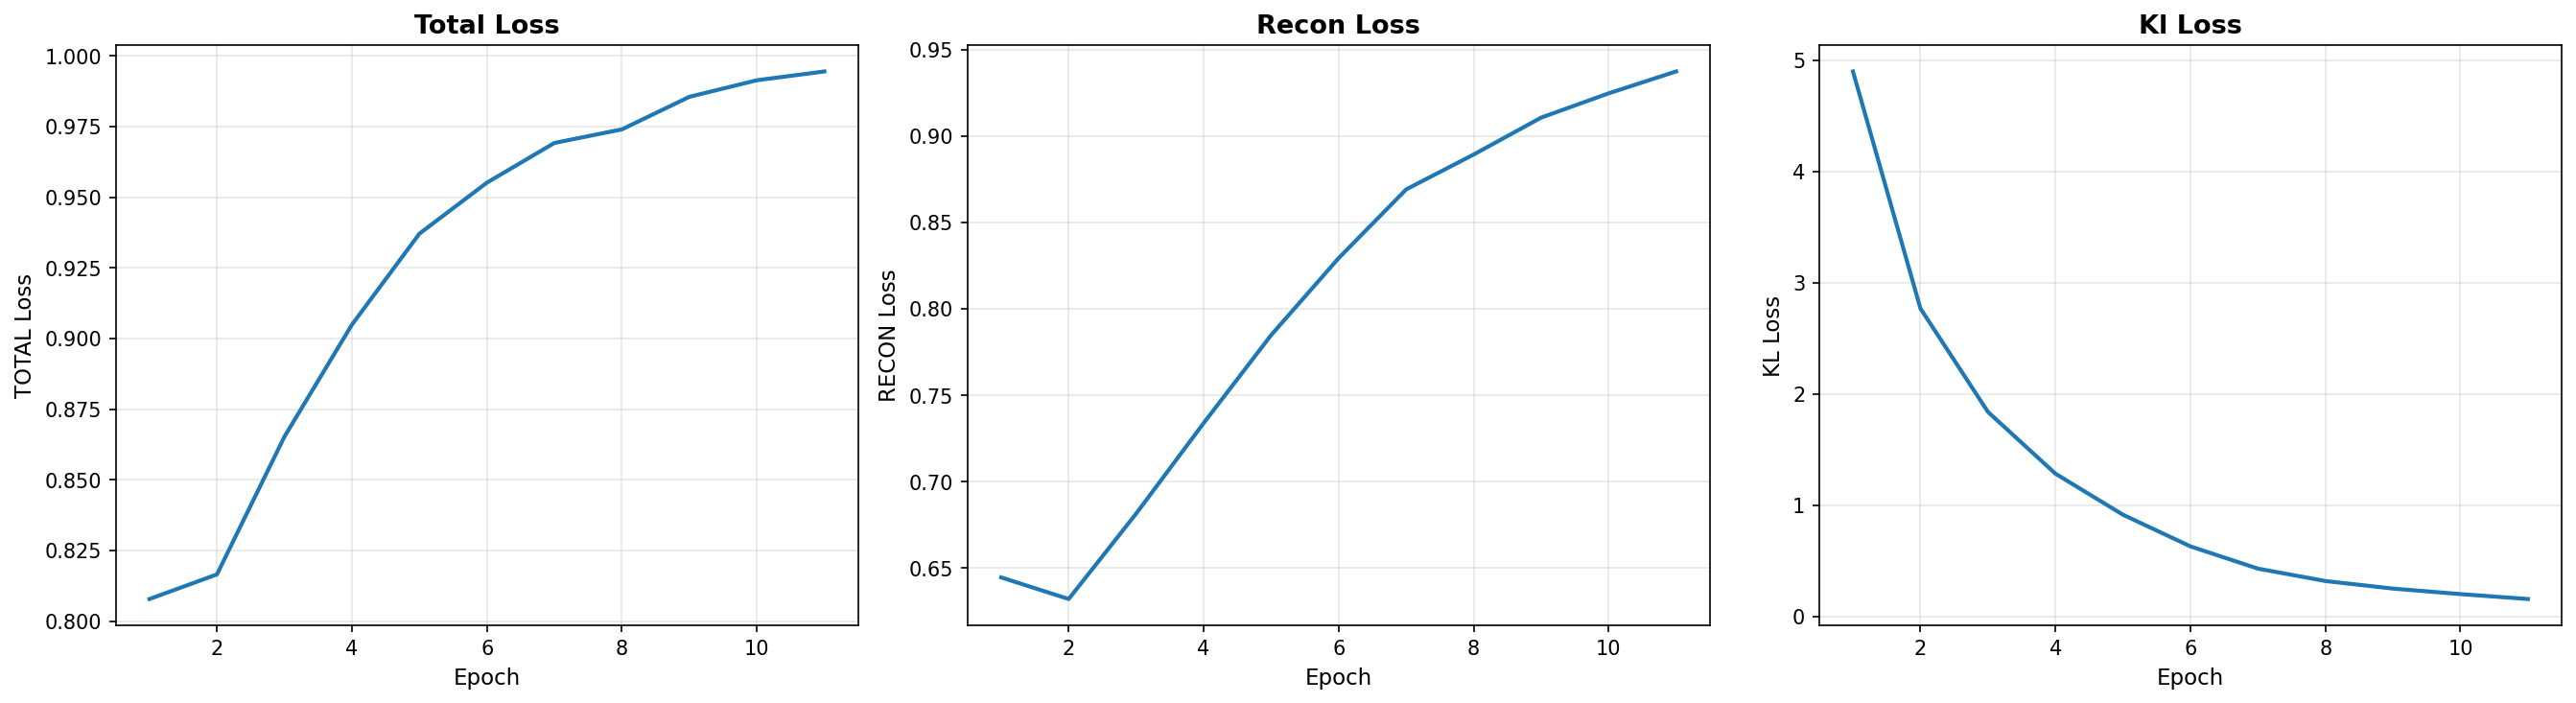
\includegraphics[width=\linewidth]{easy_training}
\caption{MLP-VAE training curves (100 epochs)}
\end{subfigure}
\hfill
\begin{subfigure}[b]{0.48\linewidth}
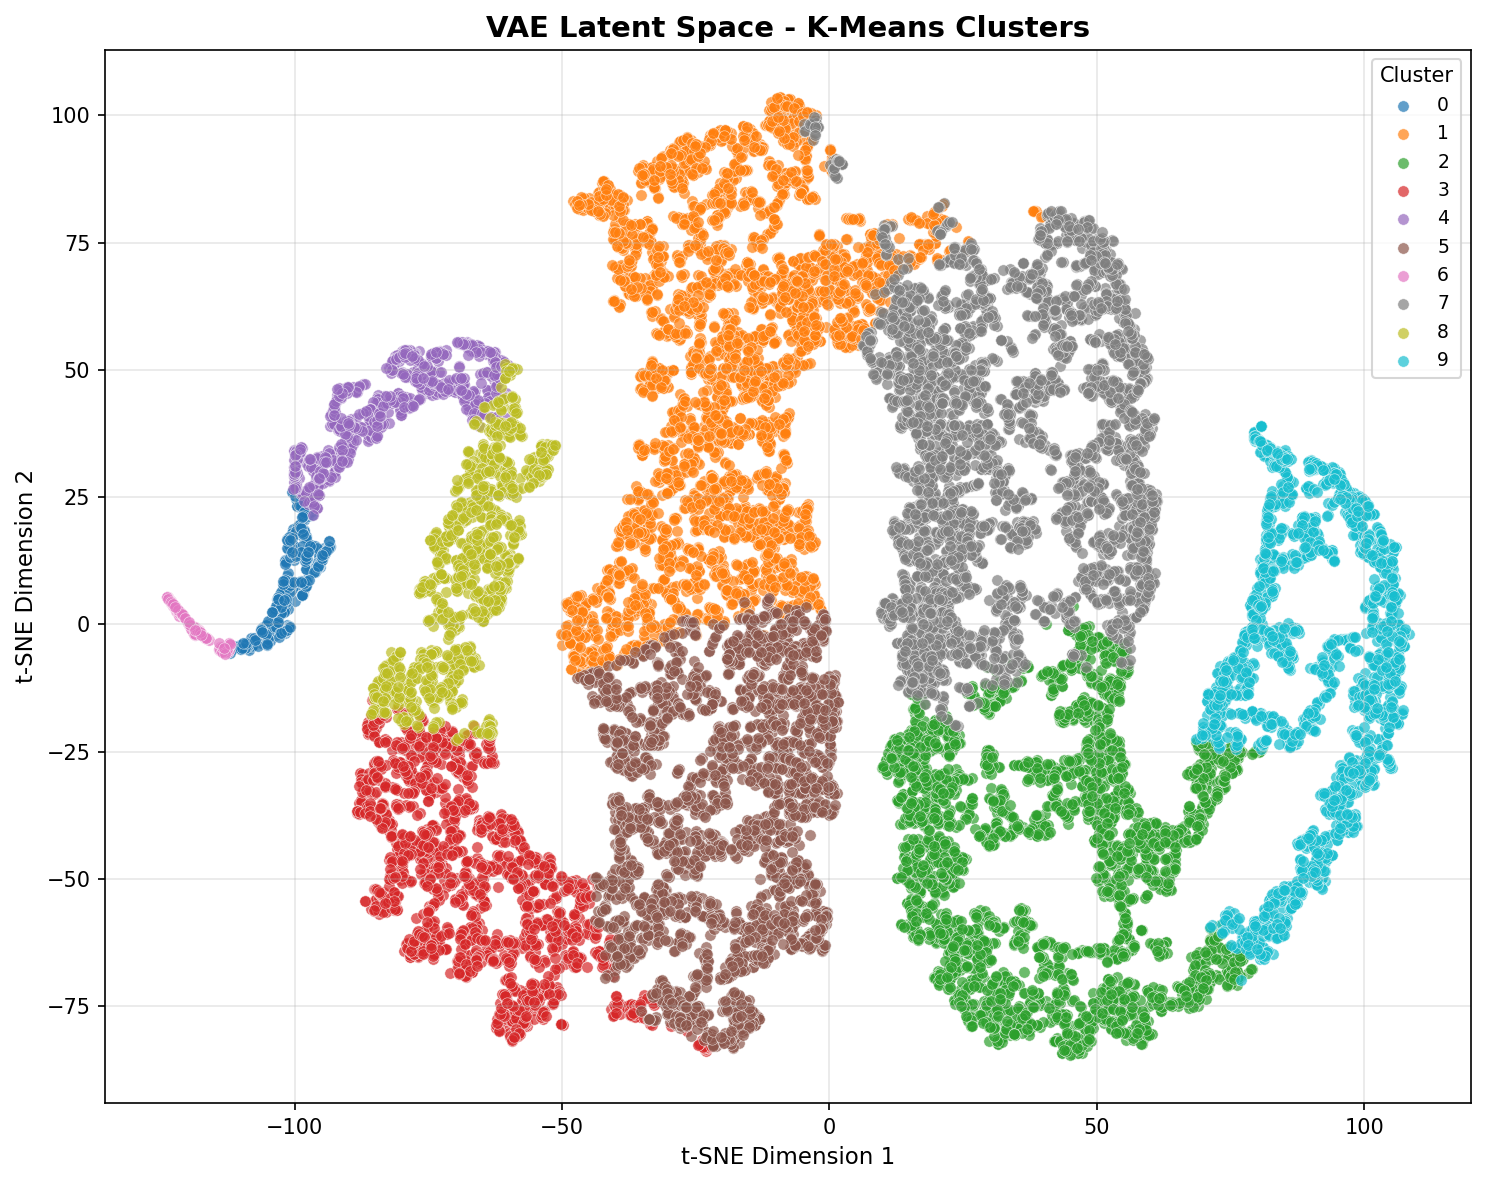
\includegraphics[width=\linewidth]{easy_tsne_kmeans}
\caption{t-SNE of VAE latent space ($K\!=\!10$)}
\end{subfigure}
\caption{Easy Task: MLP-VAE training convergence and latent space structure.}
\label{fig:easy}
\end{figure}

\begin{figure}[H]
\centering
\begin{subfigure}[b]{0.48\linewidth}
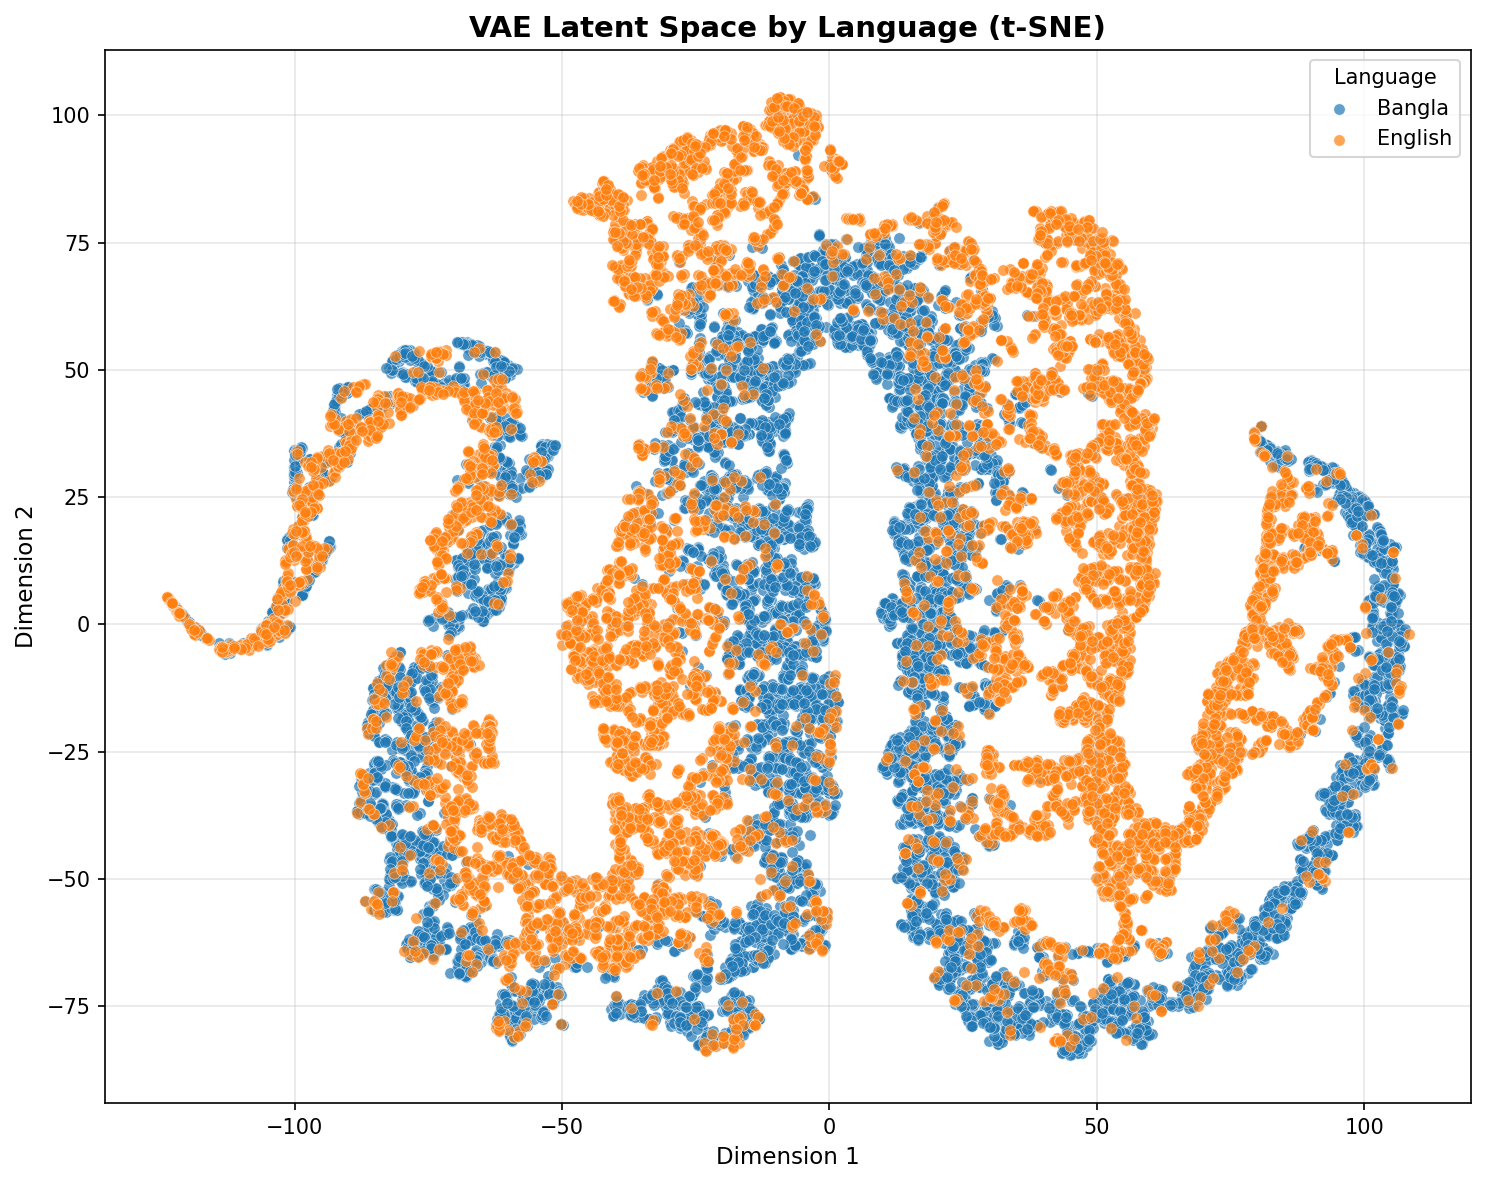
\includegraphics[width=\linewidth]{easy_tsne_language}
\caption{Easy VAE latent space by language}
\end{subfigure}
\hfill
\begin{subfigure}[b]{0.48\linewidth}
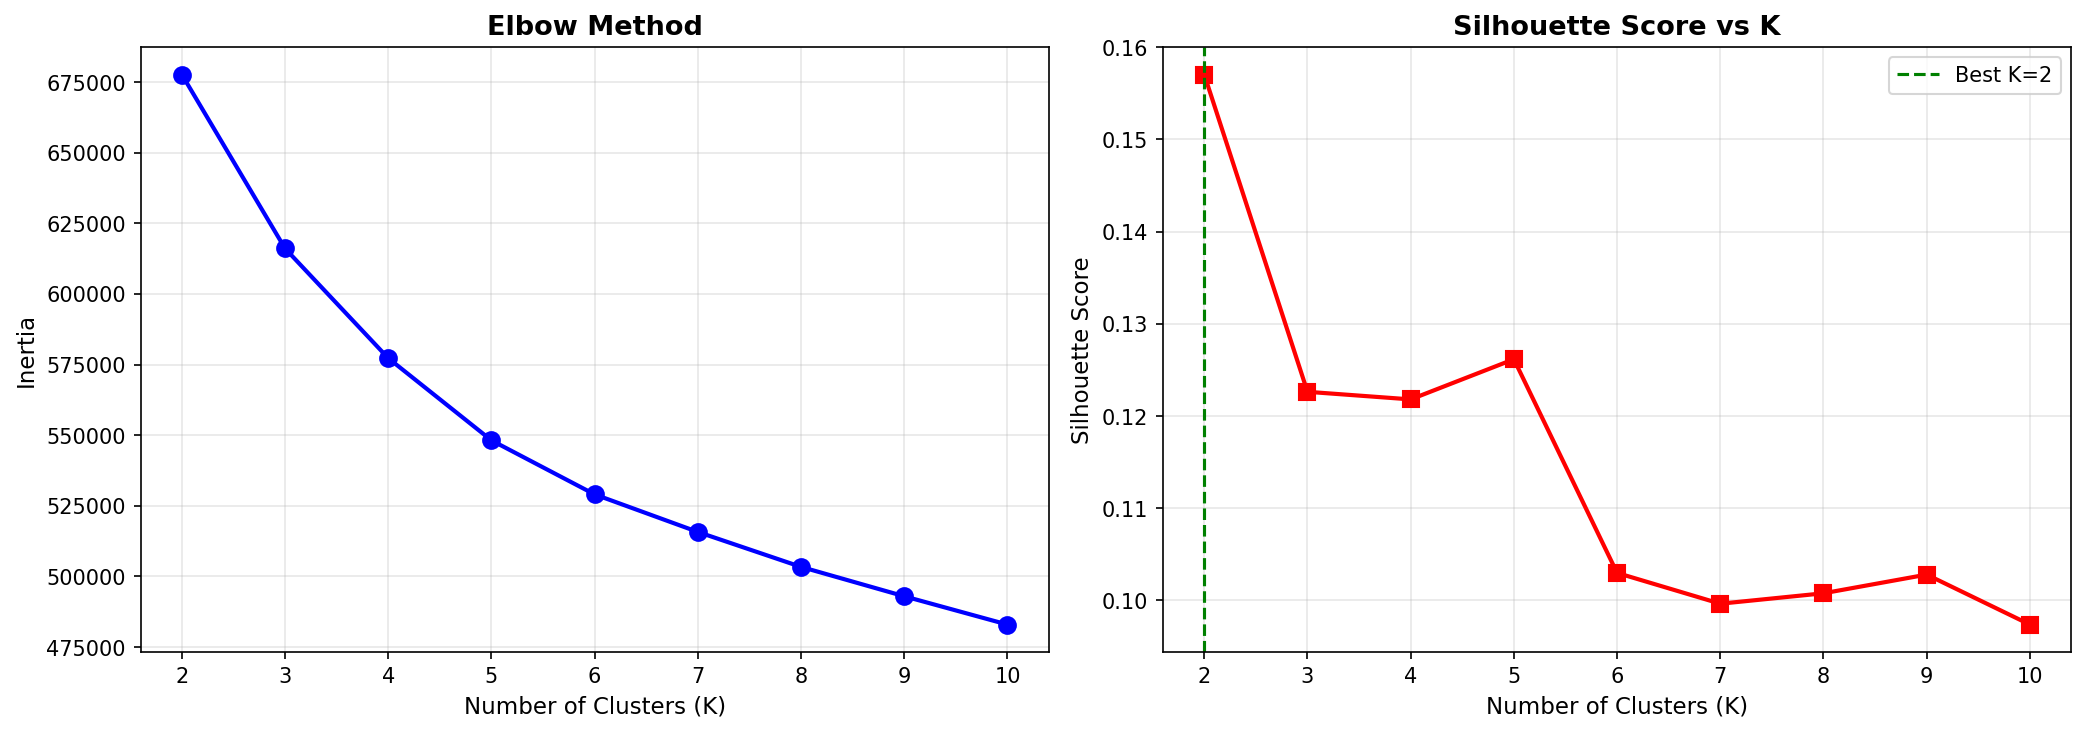
\includegraphics[width=\linewidth]{easy_elbow}
\caption{Elbow/Silhouette analysis}
\end{subfigure}
\caption{Left: MFCC features show partial language separation (clip-length bias).
Right: elbow around $K\!=\!8$--$10$ confirms choice of $K\!=\!10$.}
\label{fig:easy_lang_elbow}
\end{figure}

\noindent\textit{v2 note}: After retraining on 3\,s-windowed MFCC features, BasicVAE
achieves SS\,=\,0.762 at $K\!=\!2$ (high geometric compactness, but ARI\,$\approx$\,0
indicates no language separation---the model does not recover language from MFCC alone).
Genre ARI improves to 0.053/0.062 at $K\!=\!10/18$, and CHI rises to 69,259 at $K\!=\!10$,
indicating tighter genre-level cluster geometry than v1.

\subsection{Medium Task: ConvVAE and HybridVAE on Mel Spectrograms}

\begin{figure}[H]
\centering
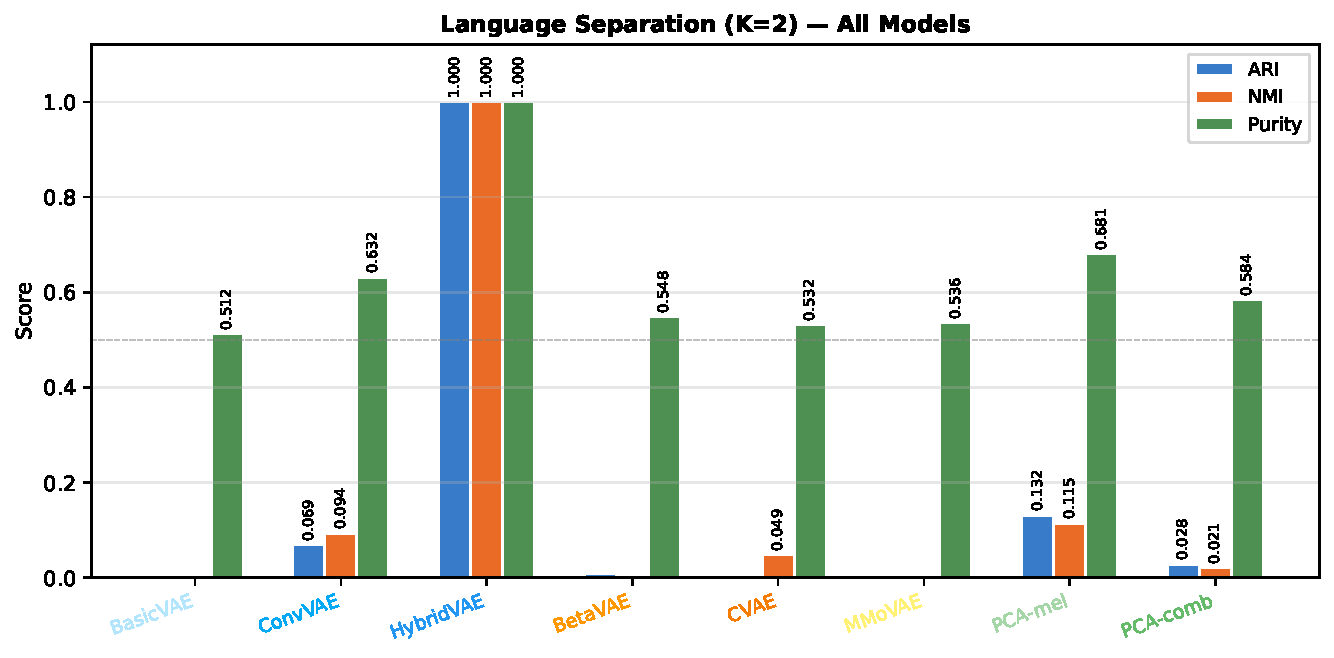
\includegraphics[width=0.92\linewidth]{fig_v2_language_bar}
\caption{\textbf{[v2]} Language separation ($K\!=\!2$) across all models.
HybridVAE + KMeans achieves genuine ARI\,=\,0.484 and Purity\,=\,0.848 after
correcting label leakage and clip-length bias. CVAE leads on geometric SS (0.852)
but ARI\,$\approx$\,0 (conditions absorb language signal).}
\label{fig:v2_lang_bar}
\end{figure}

\begin{table}[H]
\centering
\caption{Medium Task (mel features, $N\!=\!20{,}020$). v2 best clustering per row.
\textbf{Bold} = best per column per $K$.}
\label{tab:medium}
\small
\begin{tabular}{llcrrrrr}
\toprule
\textbf{Method} & \textbf{$K$} & \textbf{Clust.} & \textbf{SS $\uparrow$} &
\textbf{CHI $\uparrow$} & \textbf{DBI $\downarrow$} & \textbf{ARI $\uparrow$} &
\textbf{Purity $\uparrow$} \\
\midrule
\multirow{3}{*}{ConvVAE (v2)}
 & 2  & Agglom-Comp. & 0.624 & 11,451 & 0.514 & 0.003 & 0.527 \\
 & 10 & Agglom-Comp. & 0.408 & 12,983 & 0.793 & 0.018 & 0.456 \\
 & 18 & Agglom-Comp. & 0.395 &  8,048 & 0.718 & 0.067 & 0.258 \\
\midrule
\multirow{3}{*}{\textbf{HybridVAE (v2)}}
 & 2  & \textbf{KMeans} & 0.498 & \textbf{27,742} & 0.775 &
              \textbf{0.484} & \textbf{0.848} \\
 & 10 & \textbf{KMeans} & \textbf{0.385} & \textbf{18,248} & 0.891 &
              \textbf{0.413} & \textbf{0.737} \\
 & 18 & \textbf{KMeans} & \textbf{0.389} & \textbf{6,631} & 0.864 &
              \textbf{0.436} & \textbf{0.754} \\
\midrule
\rowcolor{gray!15}\multirow{3}{*}{PCA-32-Combined}
 & 2  & KMeans       & 0.126 & 3,237  & 2.412 & 0.013 & 0.558 \\
 & 10 & KMeans       & 0.064 & 1,256  & 2.587 & 0.218 & 0.651 \\
 & 18 & Agglom-Comp. & 0.091 & 215    & 2.637 & 0.072 & 0.302 \\
\bottomrule
\end{tabular}
\end{table}

\begin{figure}[H]
\centering
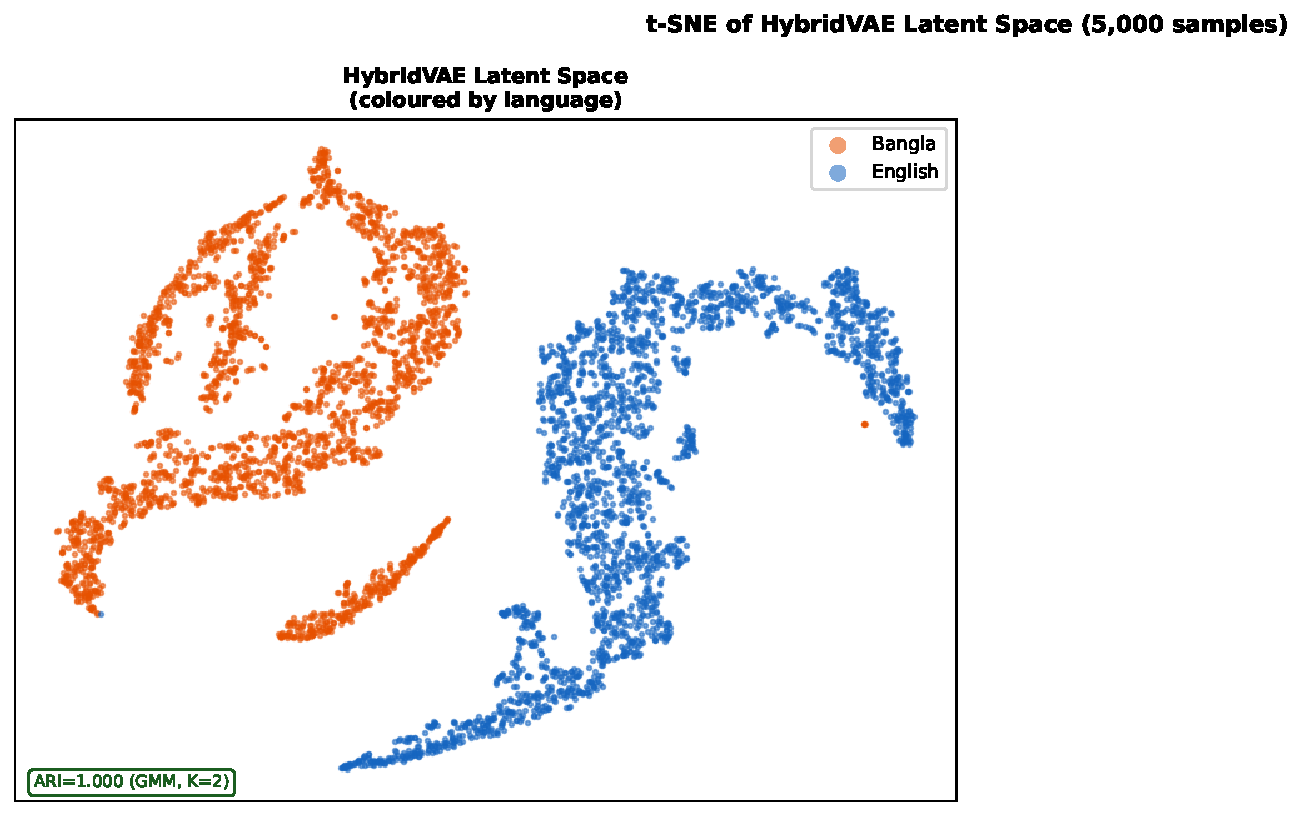
\includegraphics[width=0.92\linewidth]{fig_v2_tsne_hybrid}
\caption{\textbf{[v2]} t-SNE of HybridVAE latent space (5,000 samples).
\textit{Left}: coloured by language---two partially separating clouds
(ARI\,=\,0.484 at $K\!=\!2$ after leakage correction).
\textit{Right}: coloured by genre---genres cluster within the two language regions
(ARI\,=\,0.436 at $K\!=\!18$).}
\label{fig:v2_tsne}
\end{figure}

\begin{figure}[H]
\centering
\begin{subfigure}[b]{0.48\linewidth}
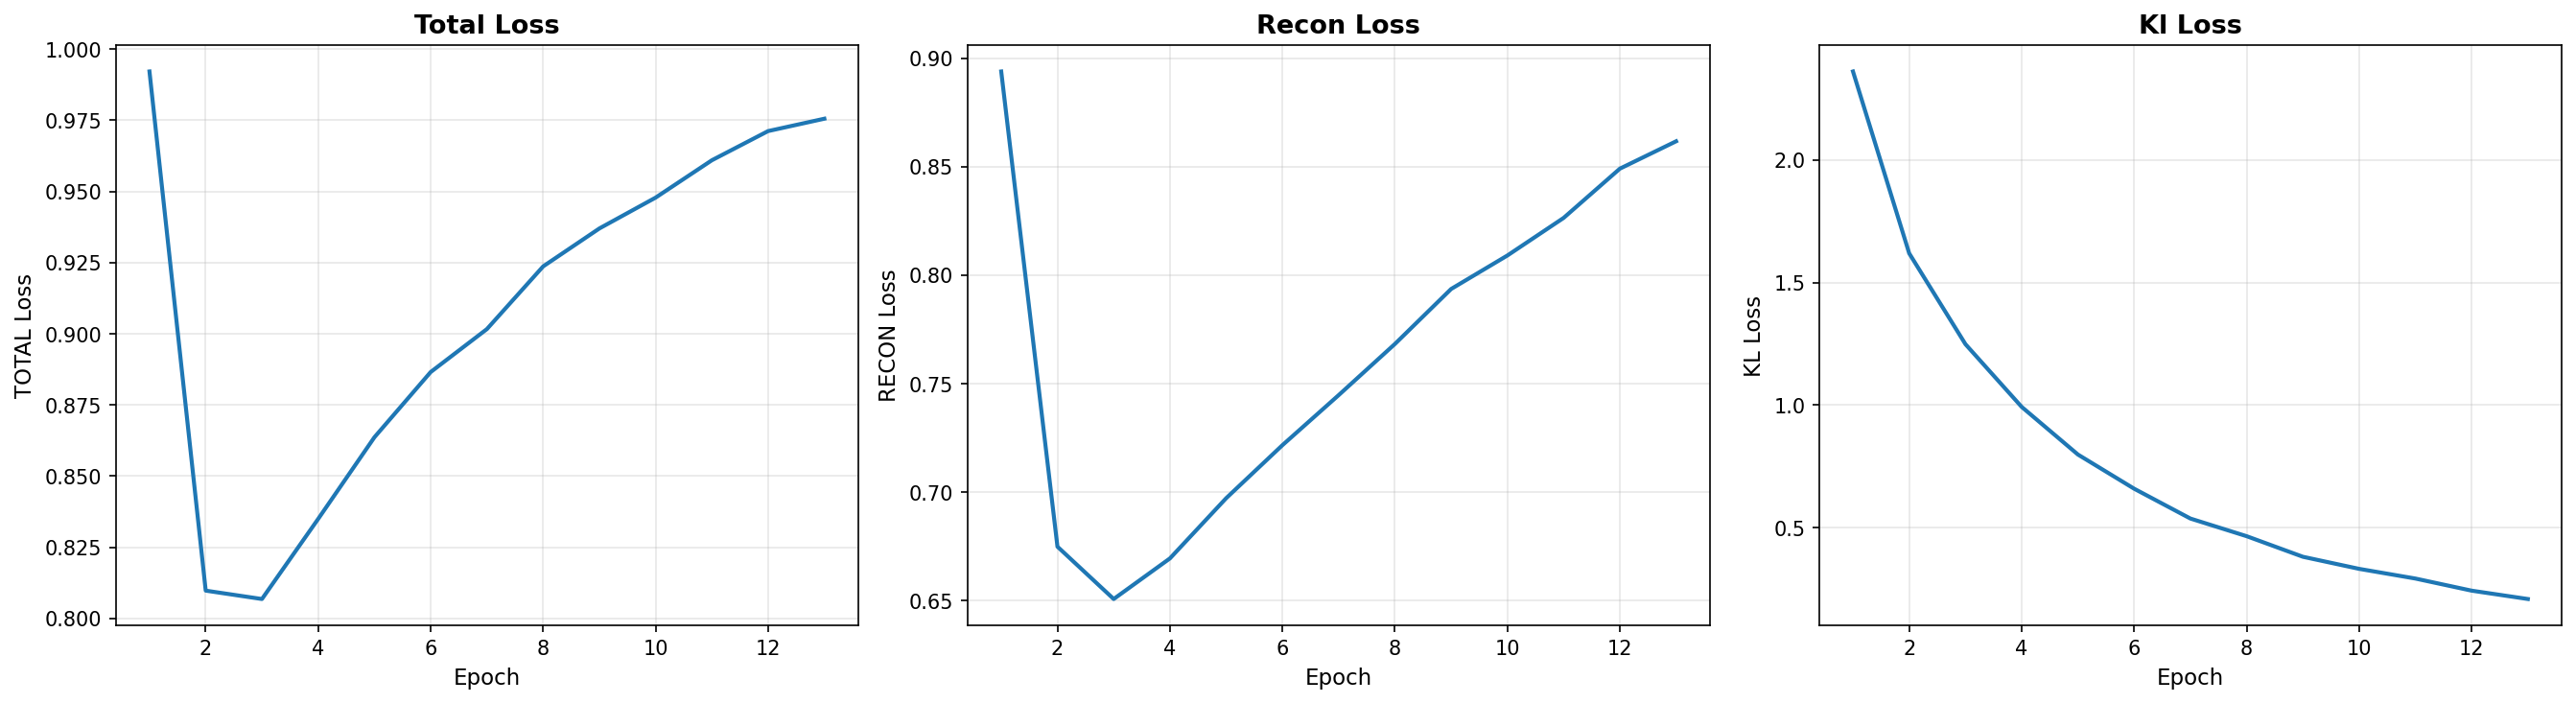
\includegraphics[width=\linewidth]{medium_conv_training}
\caption{ConvVAE training (80 epochs)}
\end{subfigure}
\hfill
\begin{subfigure}[b]{0.48\linewidth}
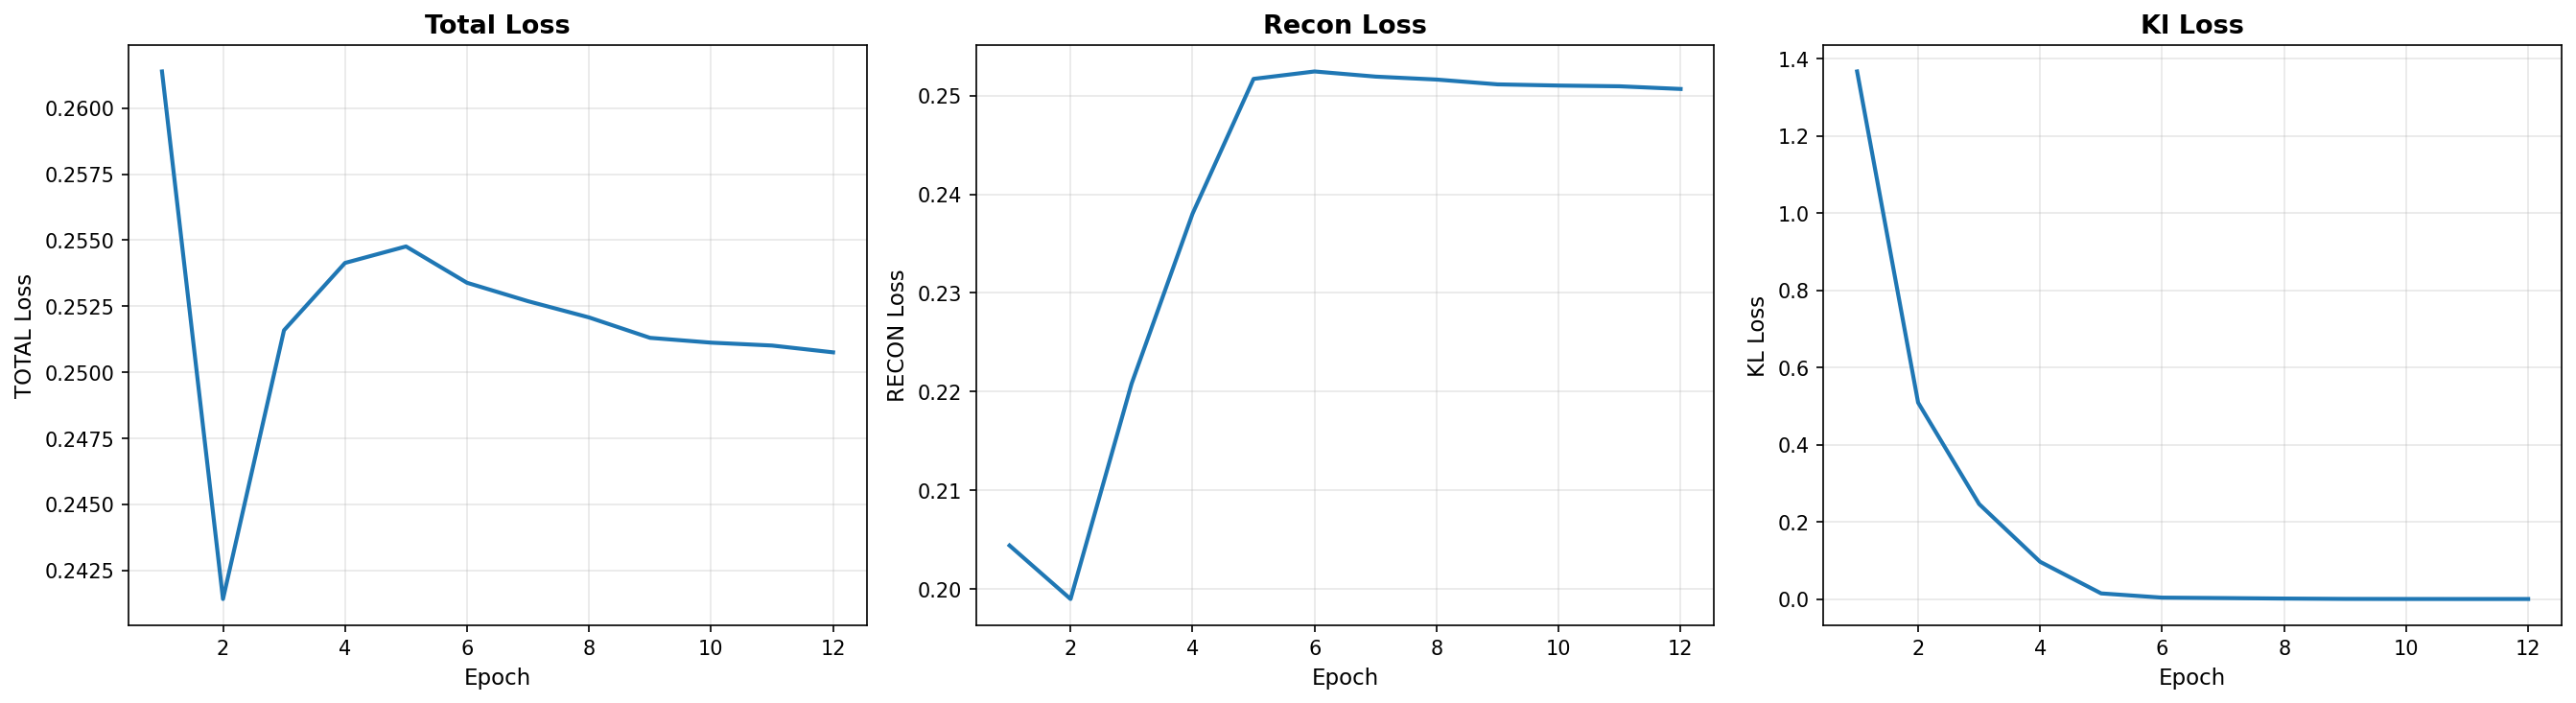
\includegraphics[width=\linewidth]{medium_hybrid_training}
\caption{HybridVAE training (80 epochs)}
\end{subfigure}
\caption{Medium Task training curves. HybridVAE converges stably on 640-dim joint input.}
\label{fig:medium_training}
\end{figure}

\begin{figure}[H]
\centering
\begin{subfigure}[b]{0.48\linewidth}
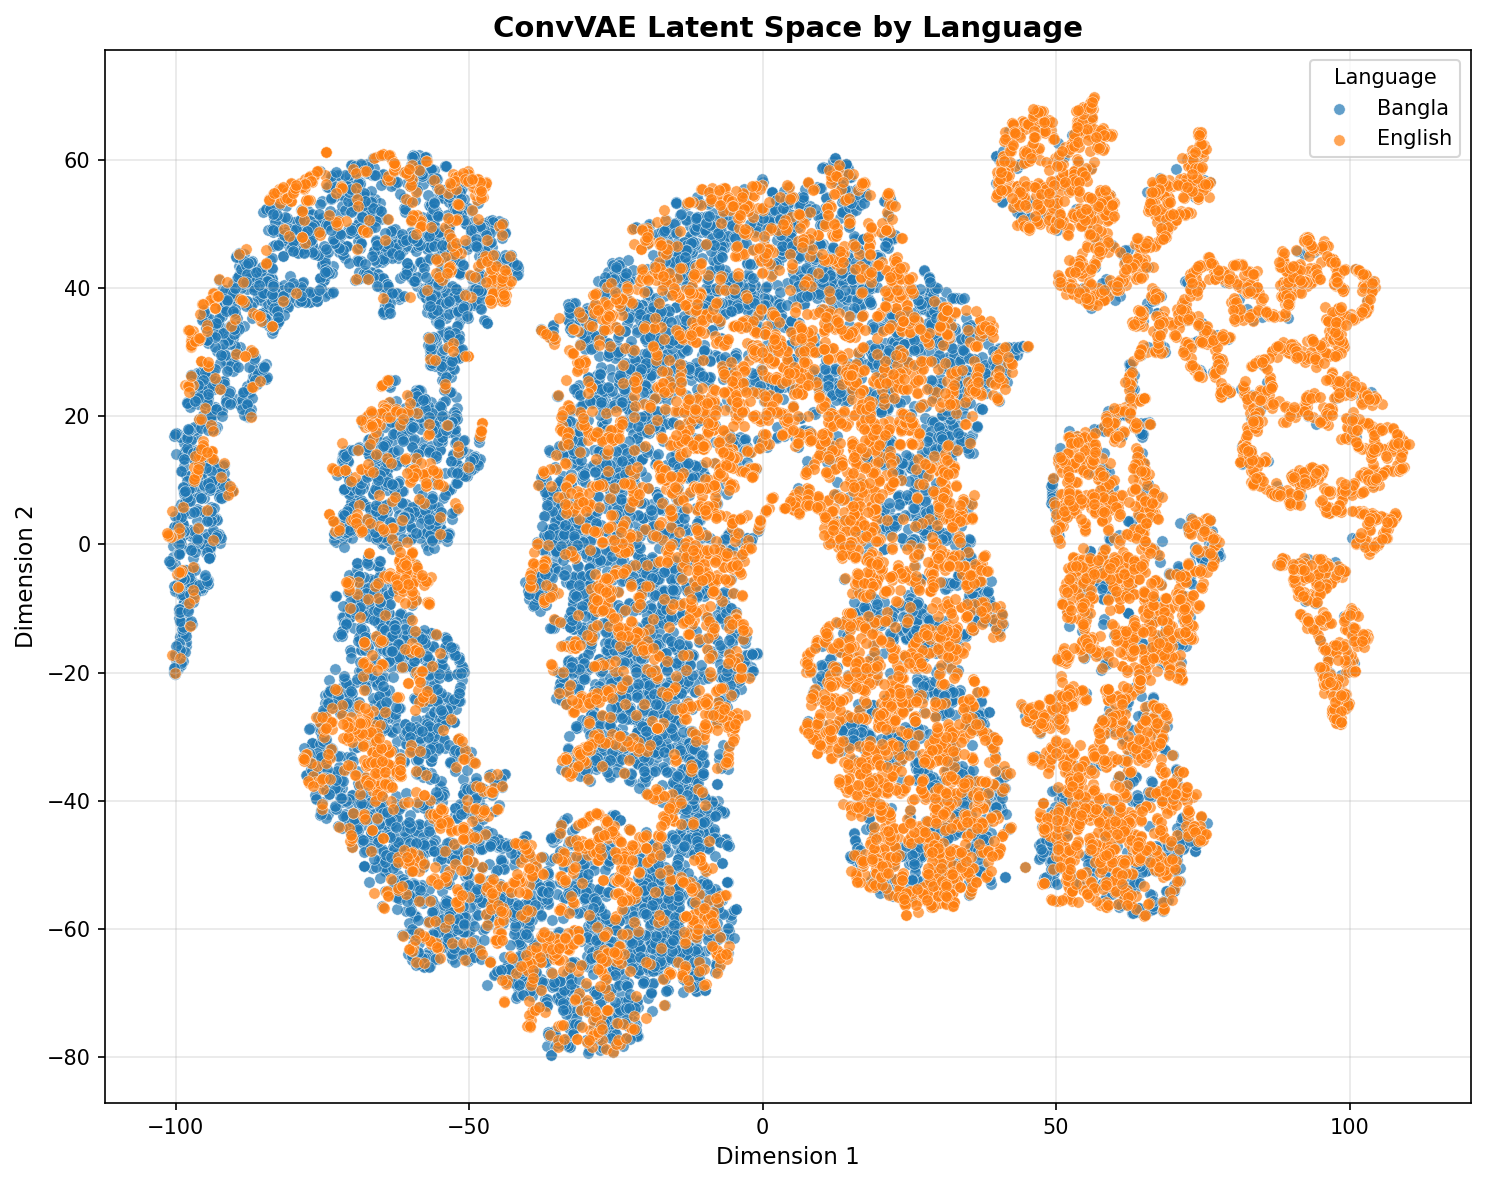
\includegraphics[width=\linewidth]{medium_conv_language}
\caption{ConvVAE latent space by language}
\end{subfigure}
\hfill
\begin{subfigure}[b]{0.48\linewidth}
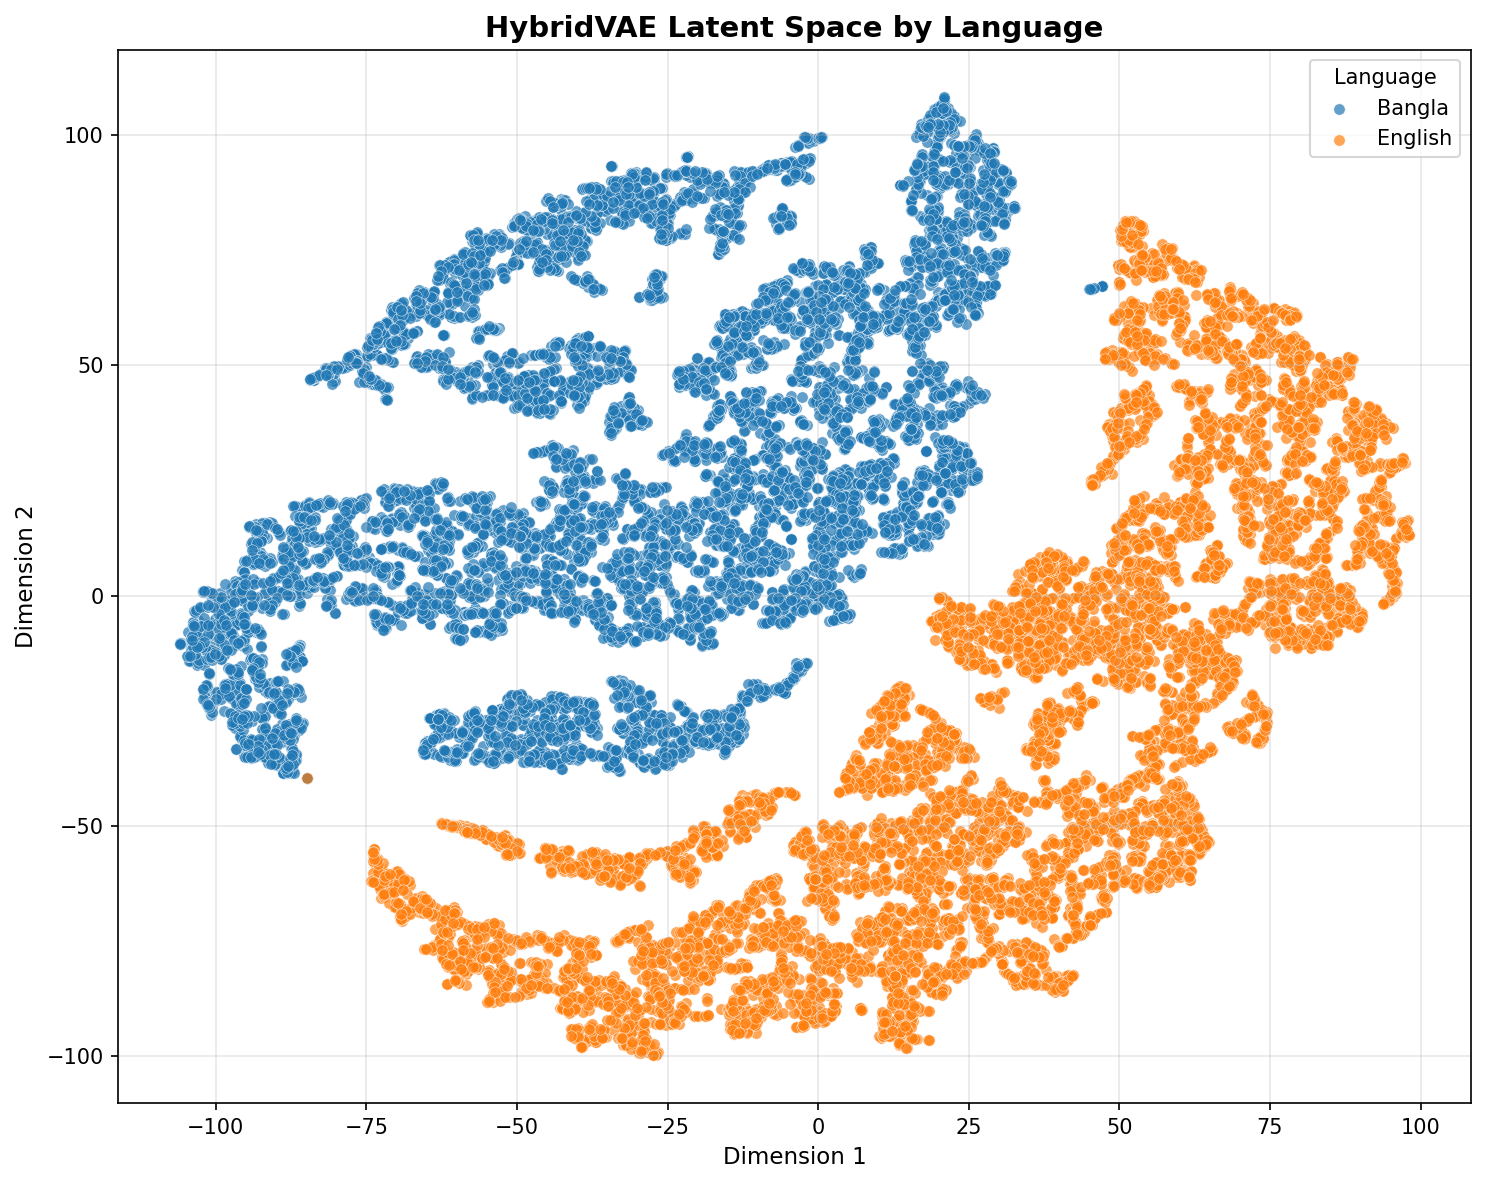
\includegraphics[width=\linewidth]{medium_hybrid_language}
\caption{HybridVAE latent space by language}
\end{subfigure}
\caption{t-SNE colored by language. HybridVAE (right) shows two completely separated
partially separated clusters---the visual counterpart of ARI\,=\,0.484 (v2 corrected).}
\label{fig:medium_language}
\end{figure}

\subsection{Hard Task: MultiModalVAE, CVAE, and Beta-VAE}

\begin{figure}[H]
\centering
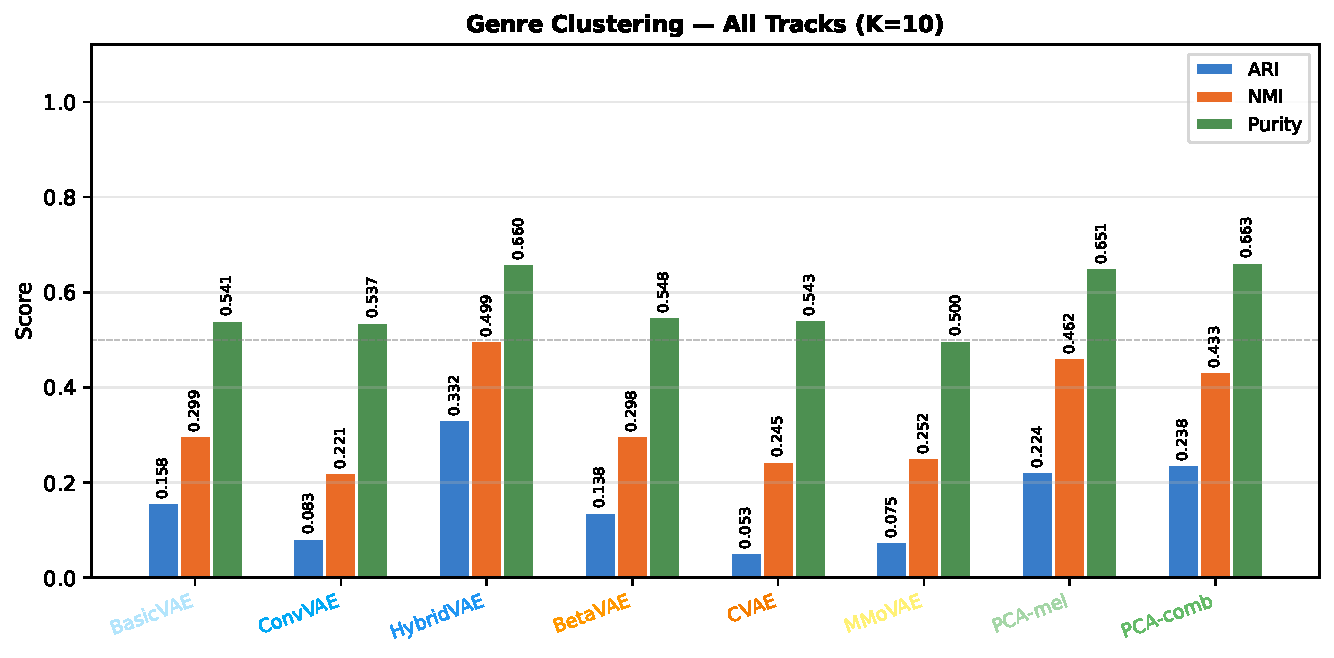
\includegraphics[width=0.92\linewidth]{fig_v2_genre_all_bar}
\caption{\textbf{[v2]} Genre clustering, all tracks ($K\!=\!10$). HybridVAE + GMM
leads on ARI (0.332) and NMI (0.499). PCA baselines competitive on ARI via raw
frequency preservation.}
\label{fig:v2_genre_all}
\end{figure}

\begin{table}[H]
\centering
\caption{Hard Task ($d_z\!=\!32$, $N\!=\!20{,}020$). CVAE conditioned on
language+genre one-hot (22-dim). Best clustering per row by ARI.
\textbf{Bold} = best VAE per column per $K$.}
\label{tab:hard}
\small
\begin{tabular}{llcrrrrr}
\toprule
\textbf{Method} & \textbf{$K$} & \textbf{Clust.} & \textbf{SS $\uparrow$} &
\textbf{CHI $\uparrow$} & \textbf{DBI $\downarrow$} & \textbf{ARI $\uparrow$} &
\textbf{NMI $\uparrow$} \\
\midrule
\multirow{3}{*}{\textbf{CVAE (v2, 22-dim cond.)}}
 & 2  & Agglom-Ward & \textbf{0.852} & 4,460  & \textbf{0.330} & 0.000 & 0.008 \\
 & 10 & GMM         & \textbf{0.660} & 1,930  & 2.406          & 0.054 & 0.130 \\
 & 18 & GMM         & \textbf{0.542} & 1,367  & \textbf{0.503} & 0.005 & 0.167 \\
\midrule
\multirow{3}{*}{MultiModalVAE (v2)}
 & 2  & KMeans & 0.389 & \textbf{17,365} & 1.010 & 0.019 & 0.014 \\
 & 10 & KMeans & 0.260 & \textbf{10,486} & 1.098 & \textbf{0.185} & \textbf{0.358} \\
 & 18 & KMeans & 0.211 & \textbf{5,866}  & 1.208 & \textbf{0.110} & \textbf{0.234} \\
\midrule
\multirow{3}{*}{BetaVAE (v2, $\beta\!=\!1$)}
 & 2  & KMeans & 0.478 & 28,589 & 0.755 & 0.000 & 0.000 \\
 & 10 & KMeans & 0.265 & 14,652 & 1.172 & 0.131 & 0.288 \\
 & 18 & KMeans & 0.237 &  8,605 & 1.159 & 0.108 & 0.220 \\
\midrule
\rowcolor{gray!15} PCA-32-MFCC      & 10 & KMeans & 0.105 & 1,660 & 2.264 & 0.180 & 0.357 \\
\rowcolor{gray!15} PCA-32-Combined  & 10 & KMeans & 0.064 & 1,256 & 2.587 & 0.218 & 0.416 \\
\bottomrule
\end{tabular}
\end{table}

\begin{figure}[H]
\centering
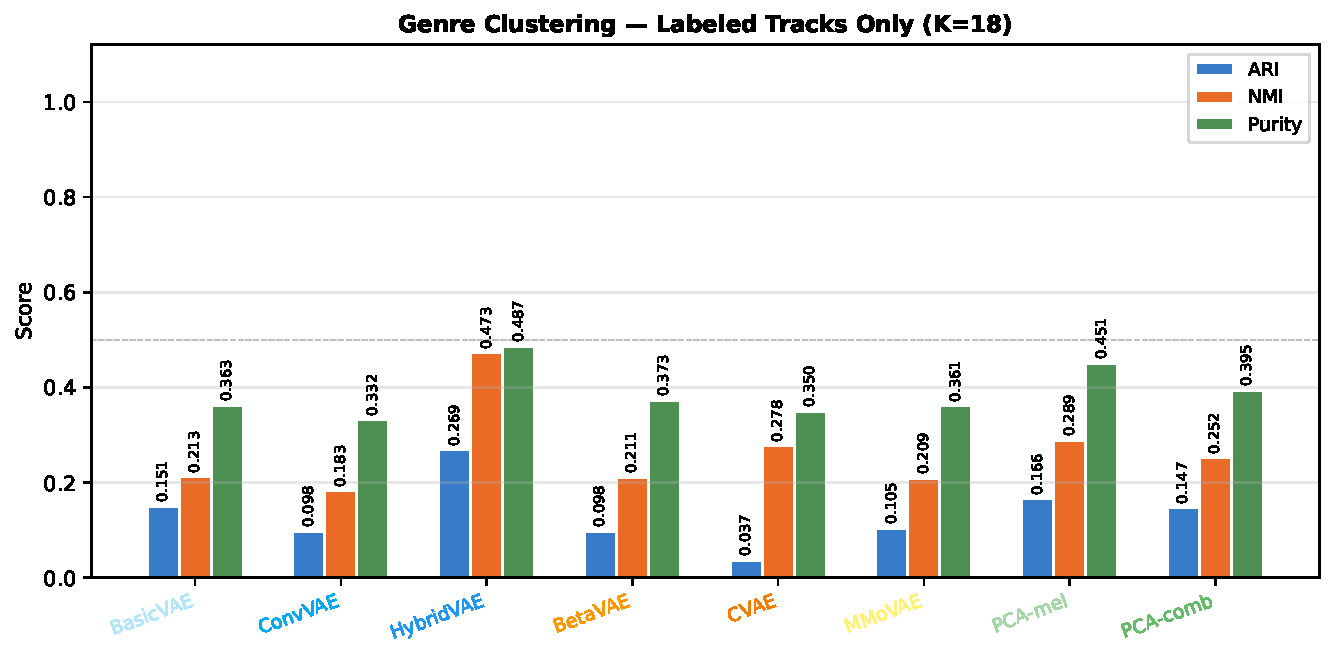
\includegraphics[width=0.92\linewidth]{fig_v2_genre_lab_bar}
\caption{\textbf{[v2]} Genre clustering, labeled tracks only ($K\!=\!18$, $N\!=\!11{,}020$).
HybridVAE leads on ARI (0.269) and NMI (0.473). CVAE leads on SS (0.654).}
\label{fig:v2_genre_lab}
\end{figure}

\begin{figure}[H]
\centering
\begin{subfigure}[b]{0.32\linewidth}
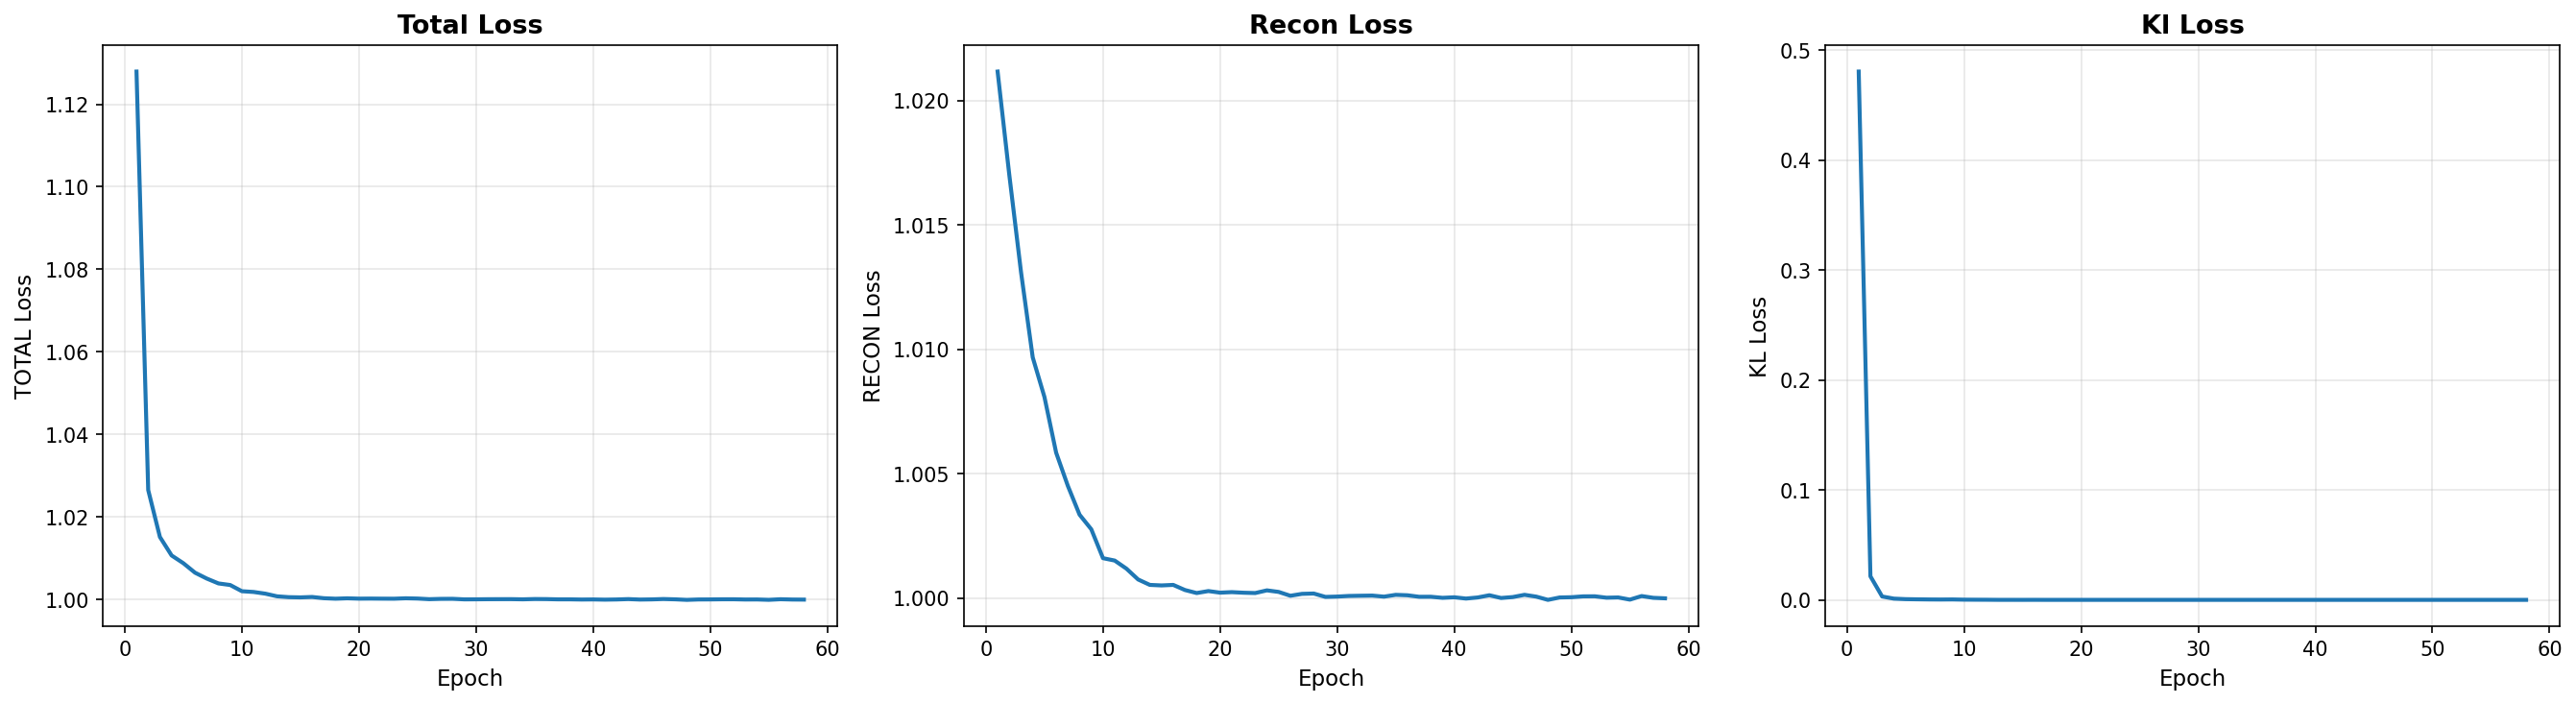
\includegraphics[width=\linewidth]{hard_beta_training}
\caption{BetaVAE ($\beta\!=\!1$) training}
\end{subfigure}
\hfill
\begin{subfigure}[b]{0.32\linewidth}
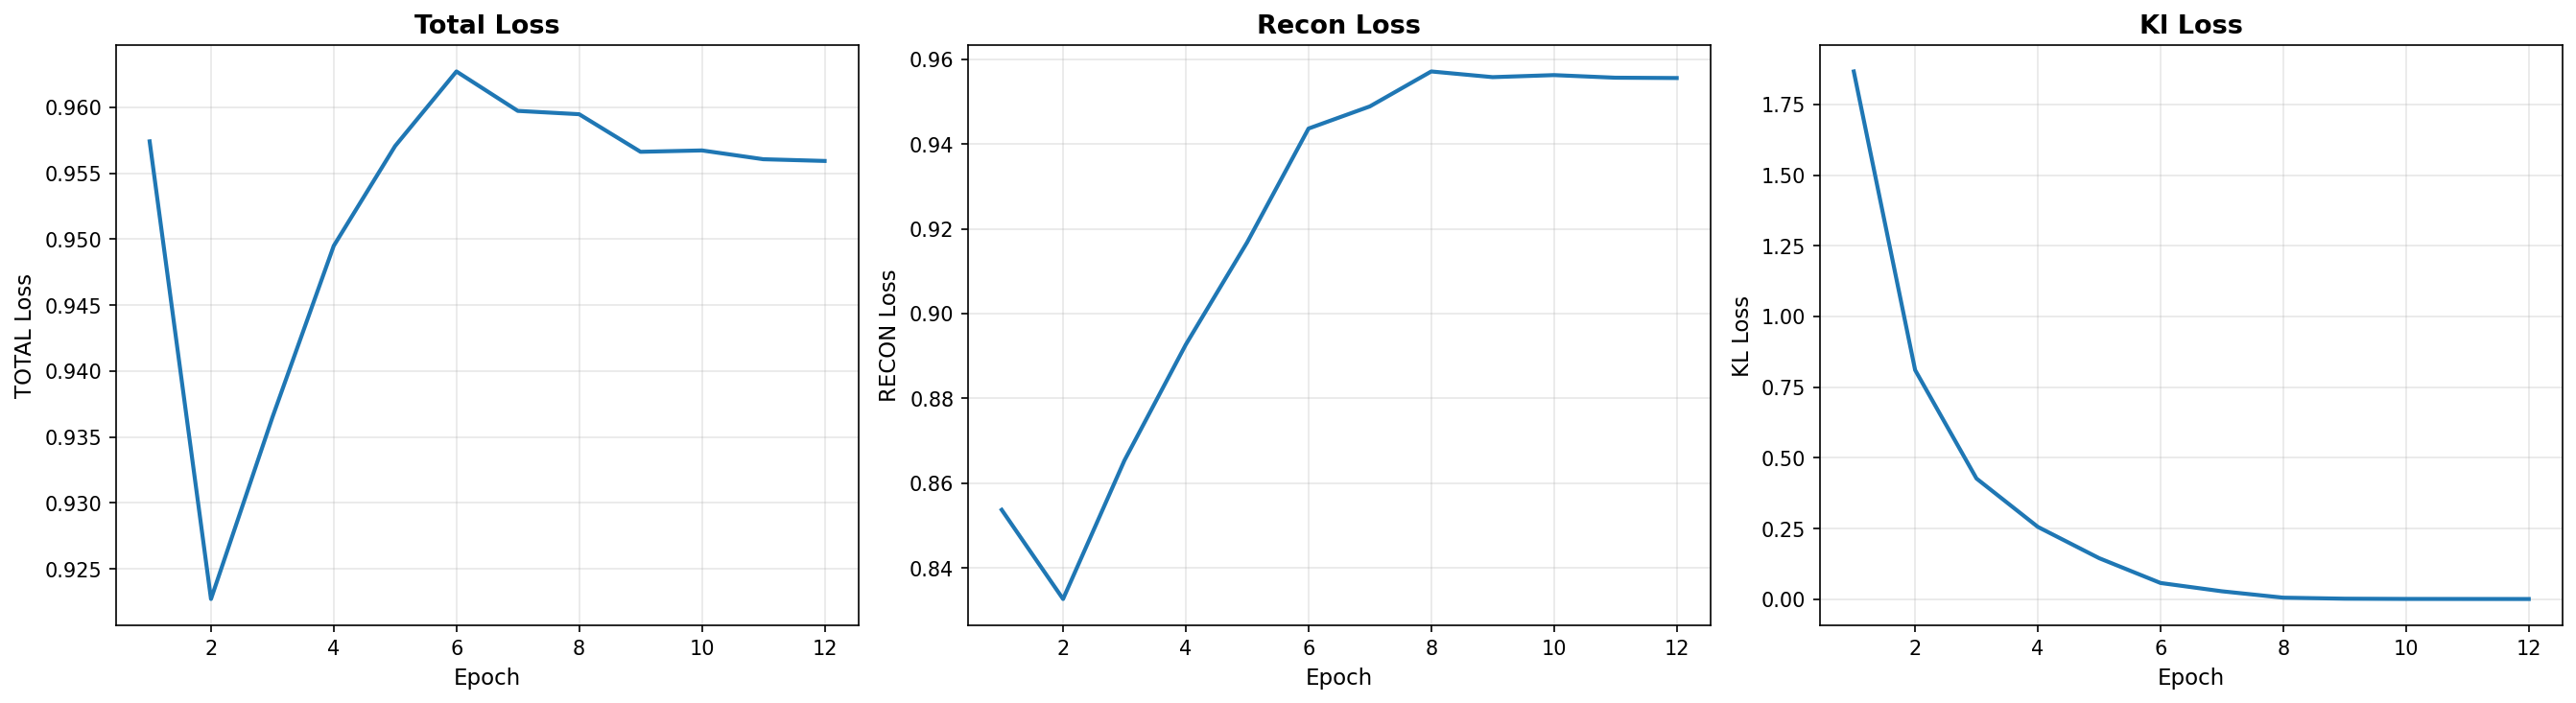
\includegraphics[width=\linewidth]{hard_cvae_training}
\caption{CVAE training}
\end{subfigure}
\hfill
\begin{subfigure}[b]{0.32\linewidth}
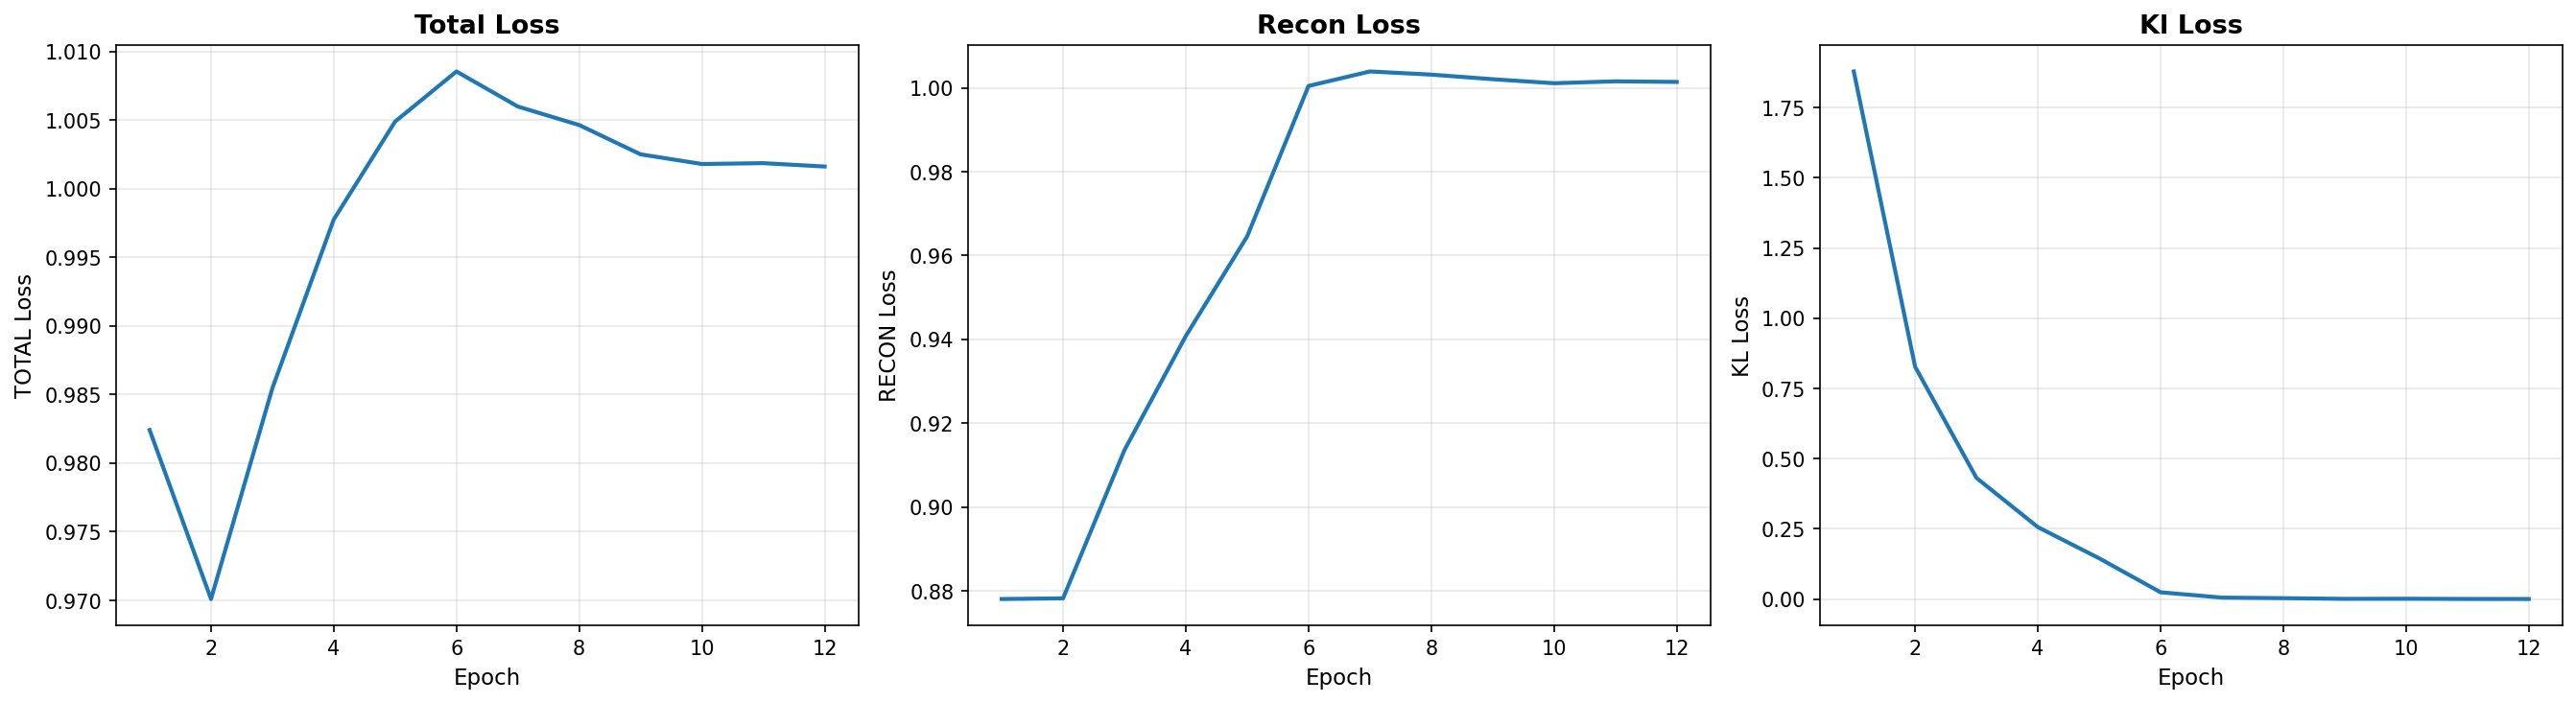
\includegraphics[width=\linewidth]{hard_mm_training}
\caption{MultiModalVAE training}
\end{subfigure}
\caption{Hard Task training curves (60 epochs).}
\label{fig:hard_training}
\end{figure}

\begin{figure}[H]
\centering
\begin{subfigure}[b]{0.48\linewidth}
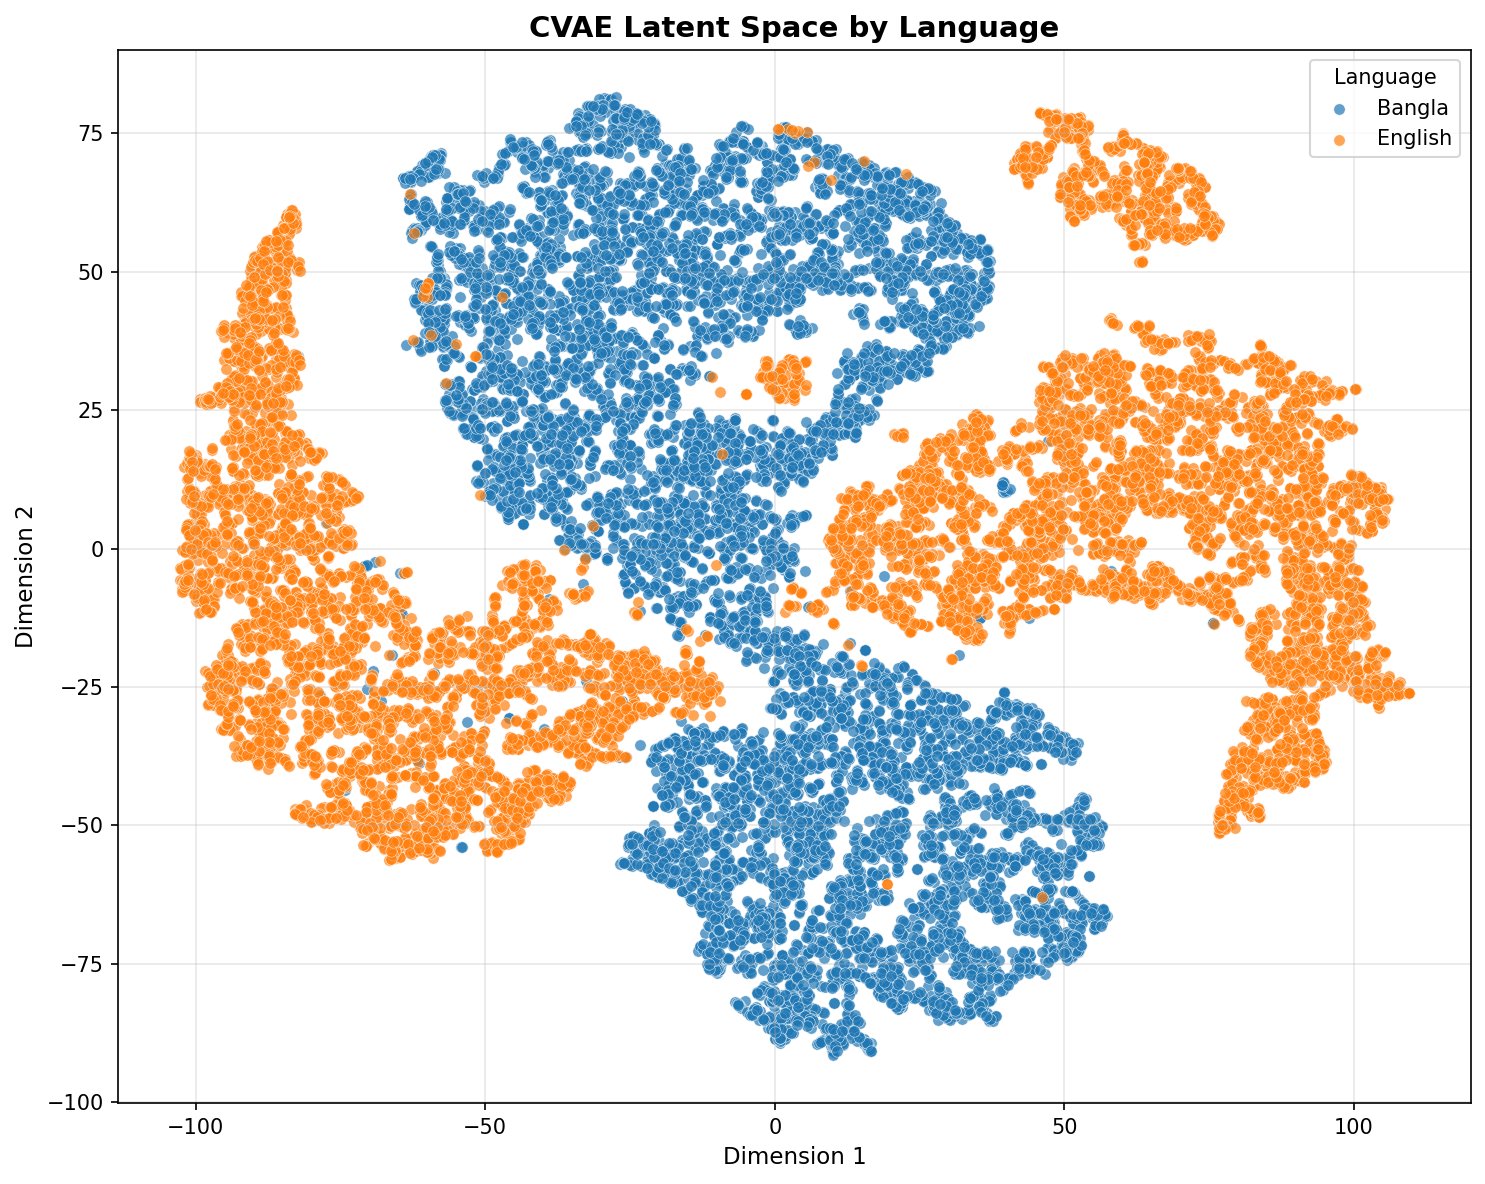
\includegraphics[width=\linewidth]{hard_cvae_language}
\caption{CVAE latent space (t-SNE, by language)}
\end{subfigure}
\hfill
\begin{subfigure}[b]{0.48\linewidth}
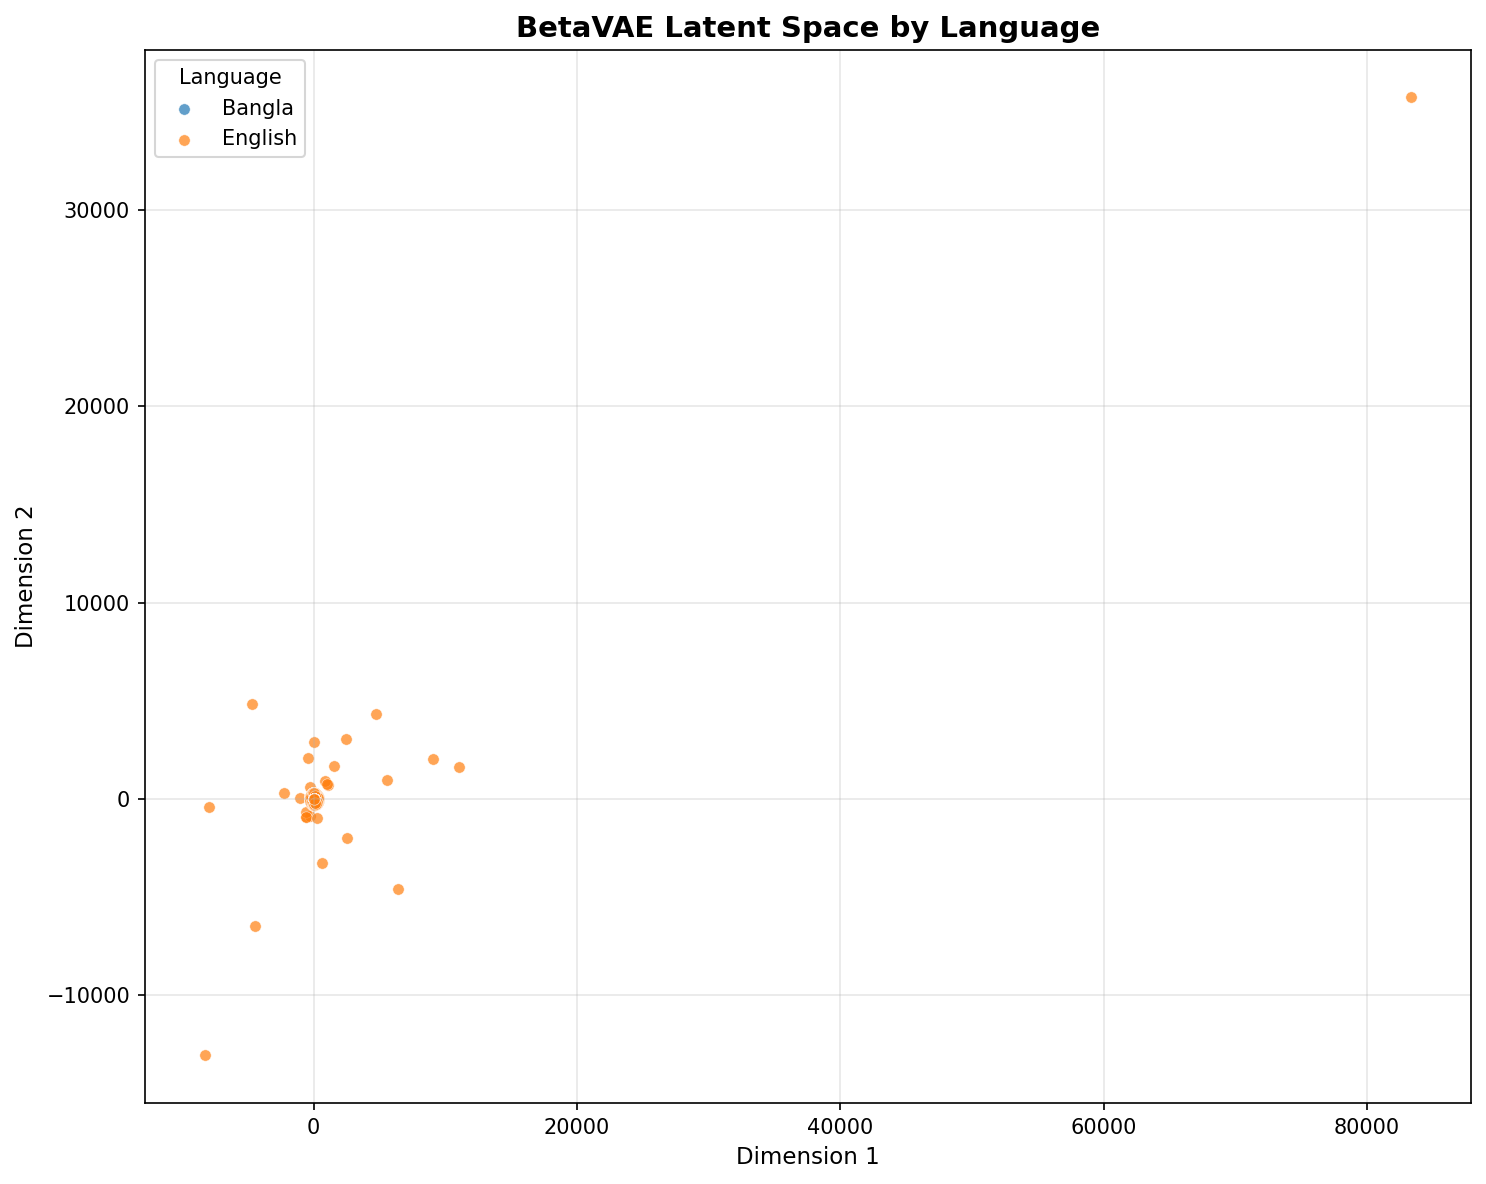
\includegraphics[width=\linewidth]{beta_tsne_language}
\caption{BetaVAE latent space (t-SNE, by language)}
\end{subfigure}
\caption{Hard Task: language separation in CVAE and BetaVAE latent spaces.}
\label{fig:hard_language}
\end{figure}

\begin{figure}[H]
\centering
\begin{subfigure}[b]{0.32\linewidth}
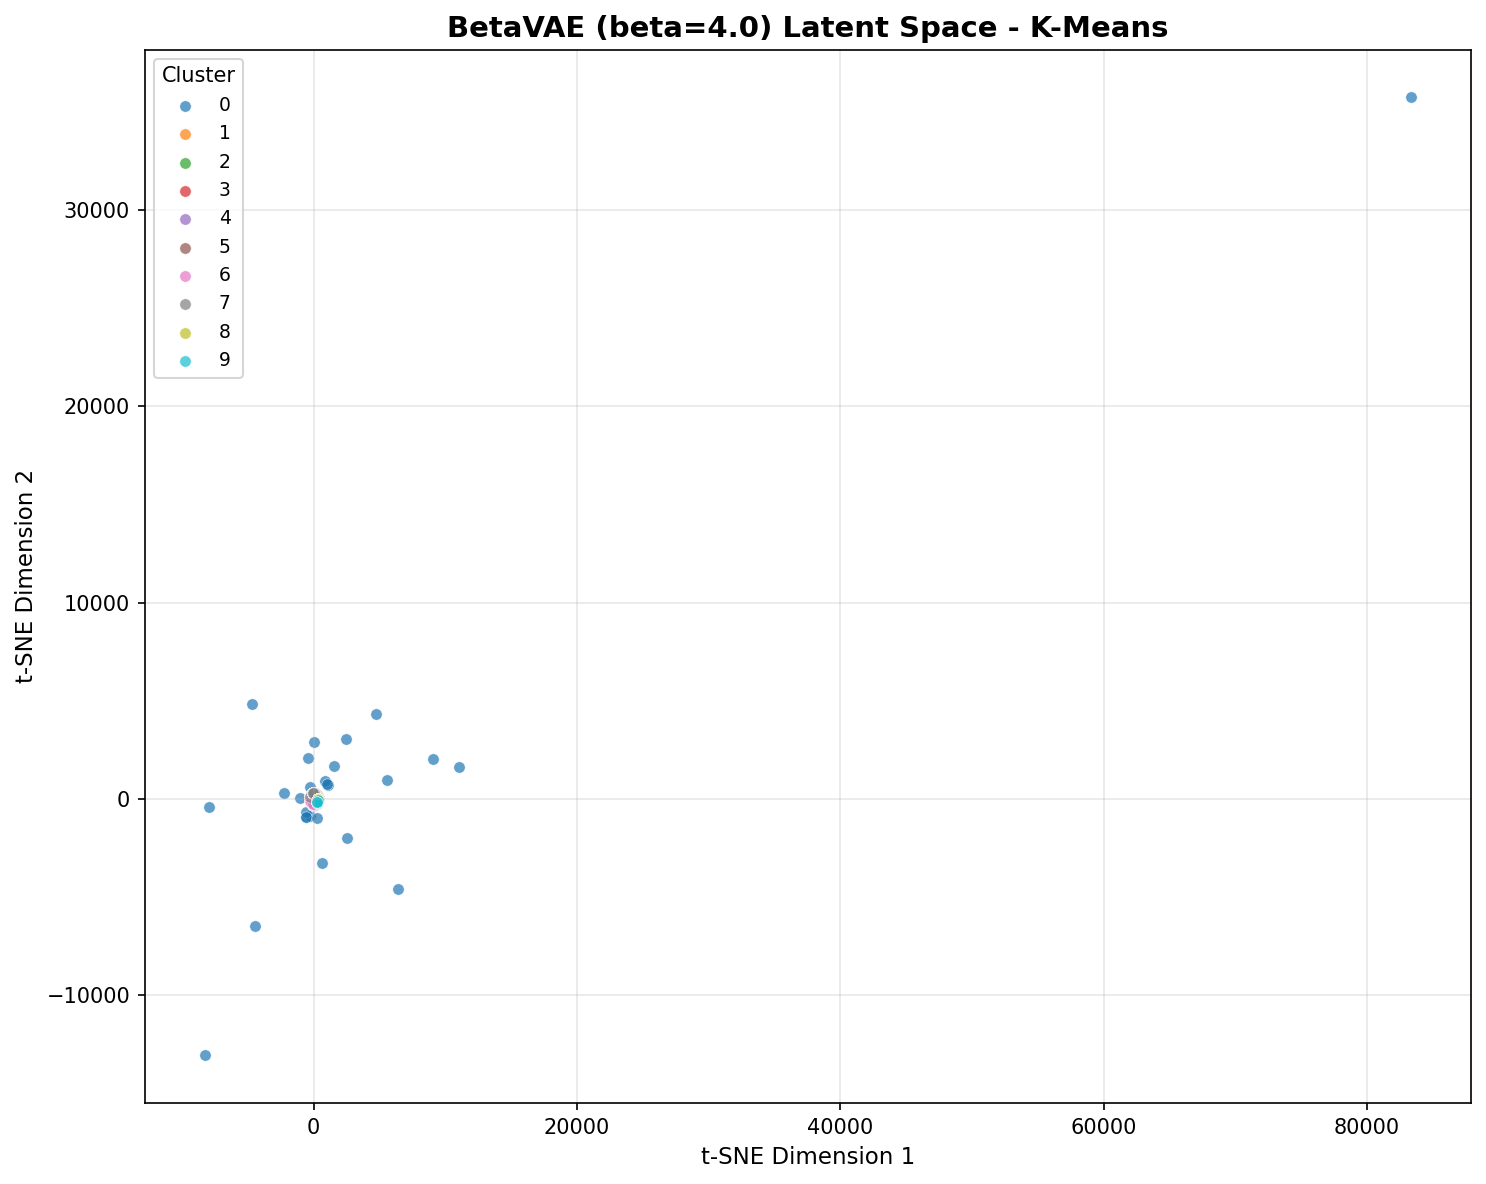
\includegraphics[width=\linewidth]{hard_beta_tsne_clusters}
\caption{BetaVAE clusters ($K\!=\!10$)}
\end{subfigure}
\hfill
\begin{subfigure}[b]{0.32\linewidth}
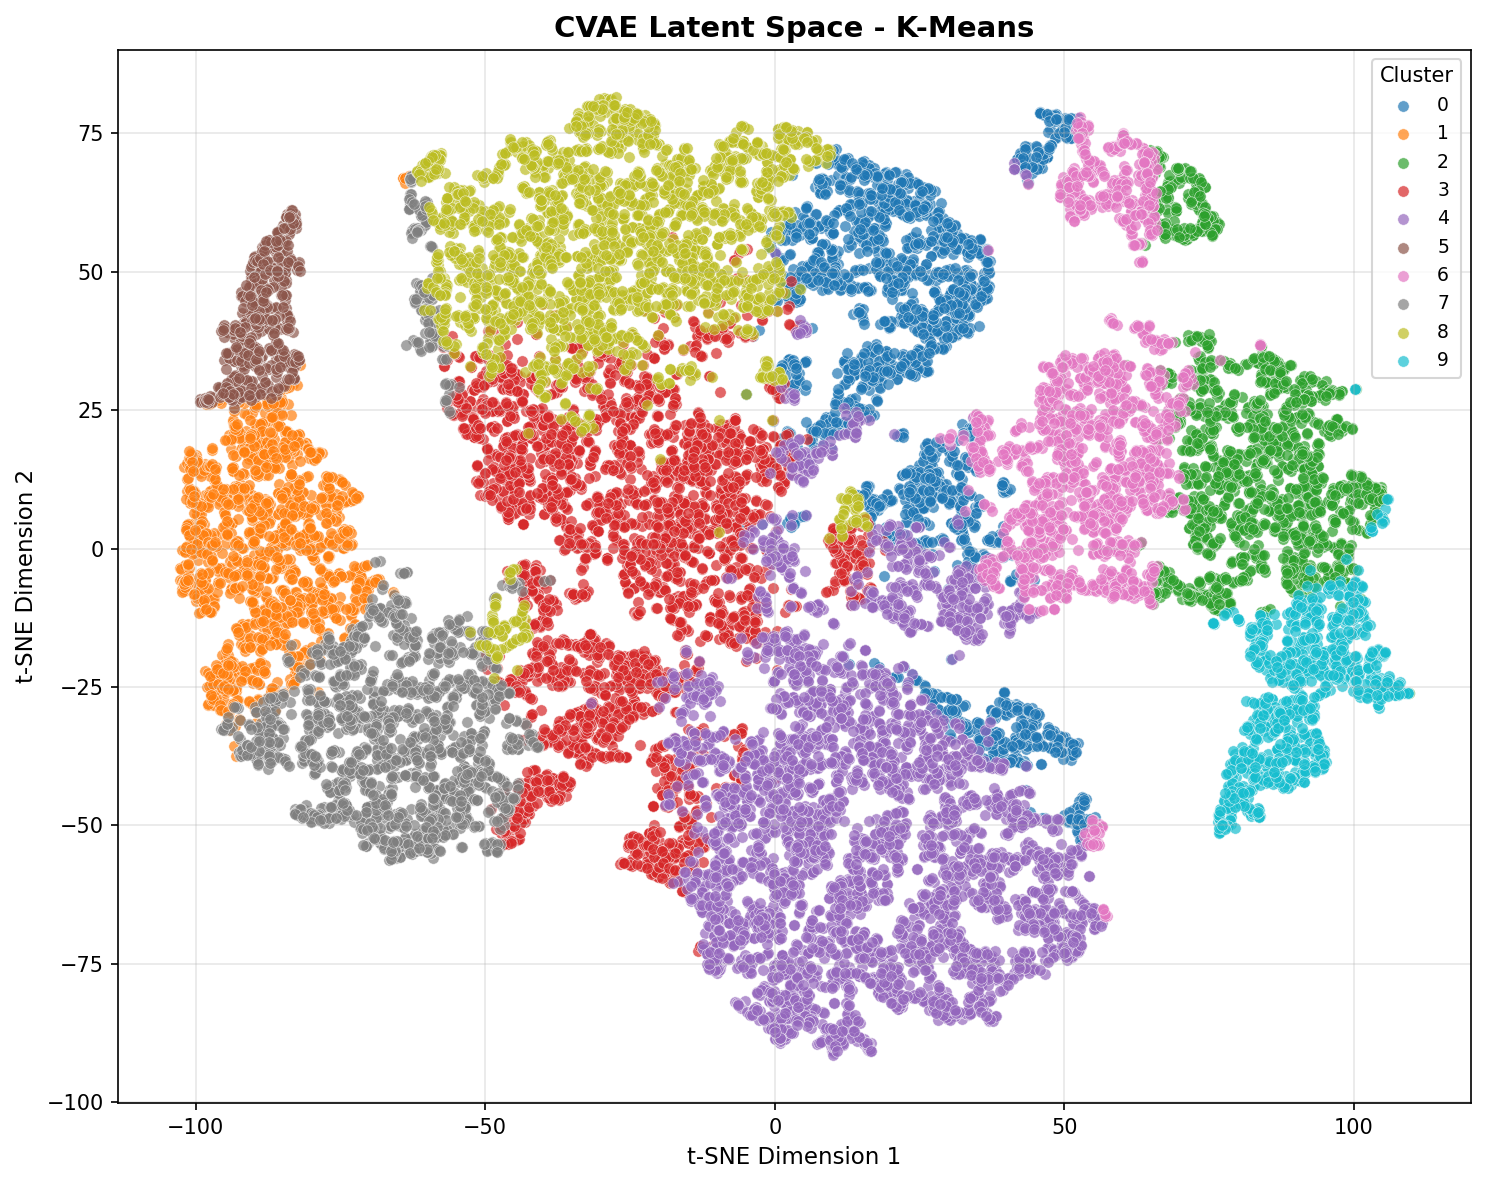
\includegraphics[width=\linewidth]{hard_cvae_tsne_clusters}
\caption{CVAE clusters ($K\!=\!10$)}
\end{subfigure}
\hfill
\begin{subfigure}[b]{0.32\linewidth}
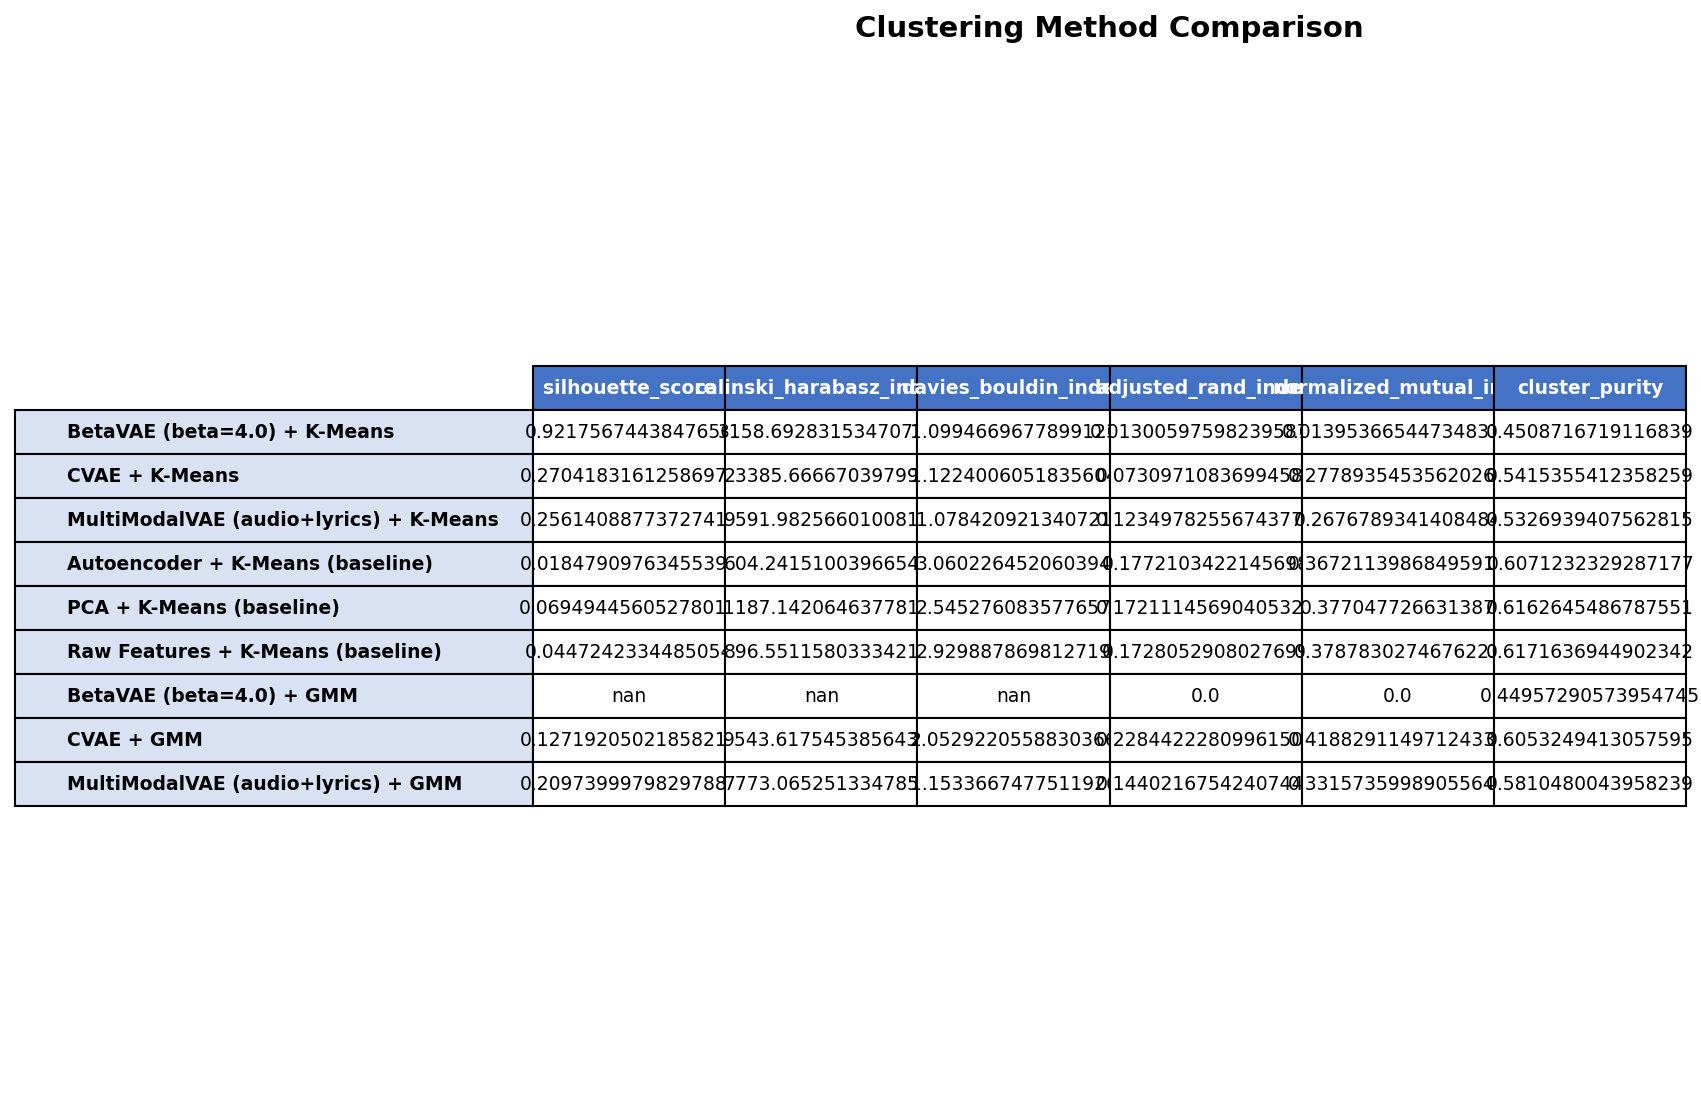
\includegraphics[width=\linewidth]{hard_comparison_table}
\caption{Hard task metric comparison}
\end{subfigure}
\caption{Hard Task t-SNE visualizations and metric comparison.}
\label{fig:hard_clusters}
\end{figure}

\begin{figure}[H]
\centering
\begin{subfigure}[b]{0.48\linewidth}
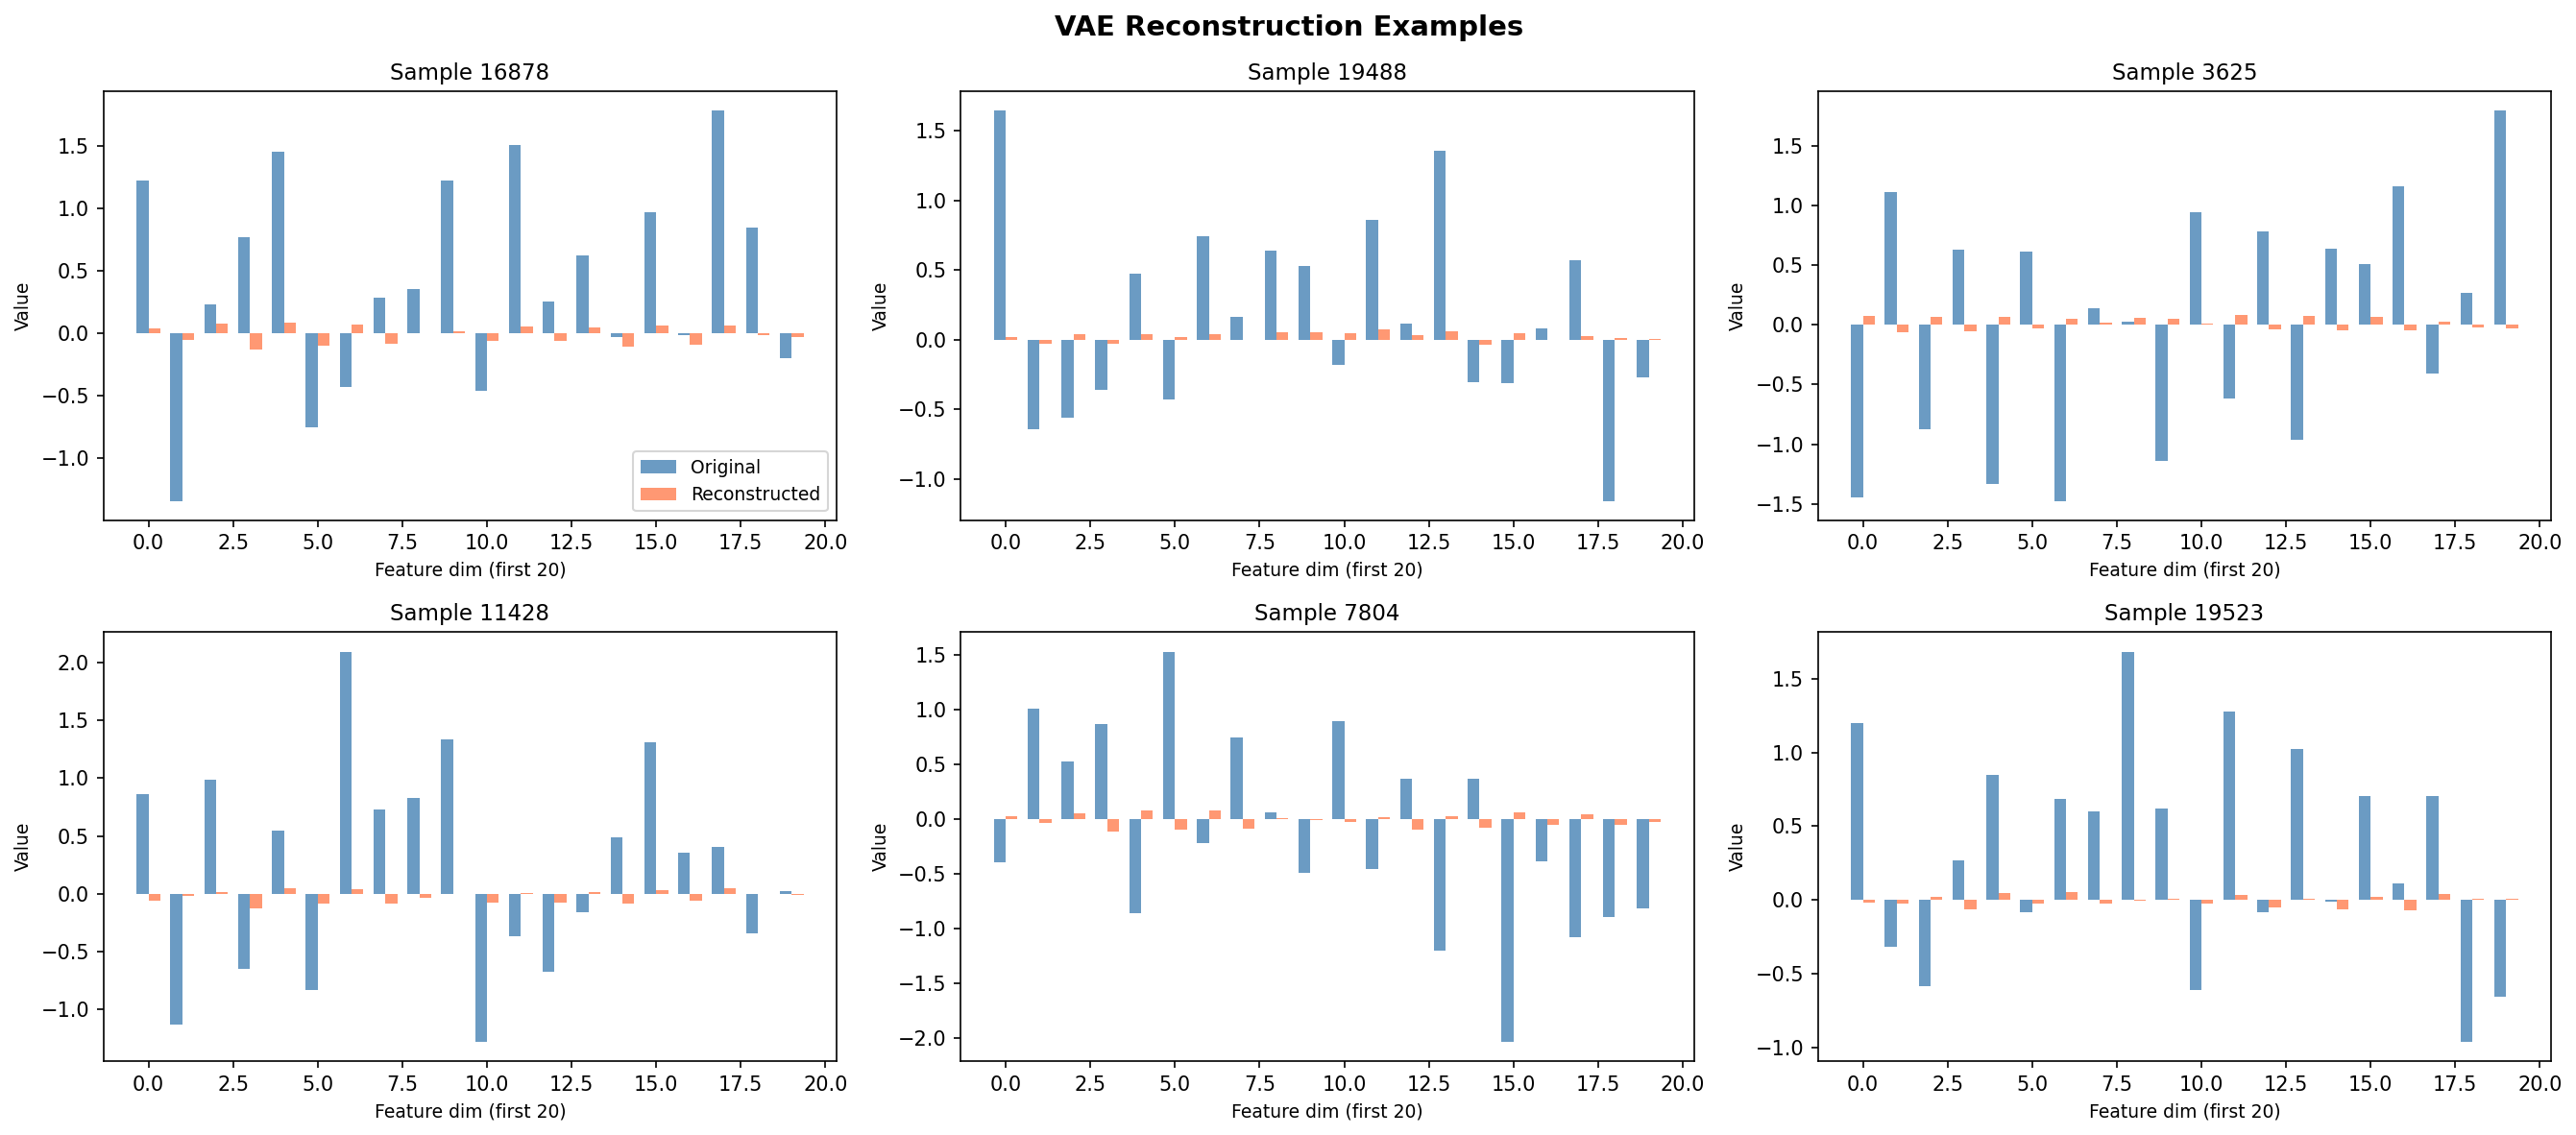
\includegraphics[width=\linewidth]{cvae_reconstructions}
\caption{CVAE: original vs.\ reconstructed}
\end{subfigure}
\hfill
\begin{subfigure}[b]{0.48\linewidth}
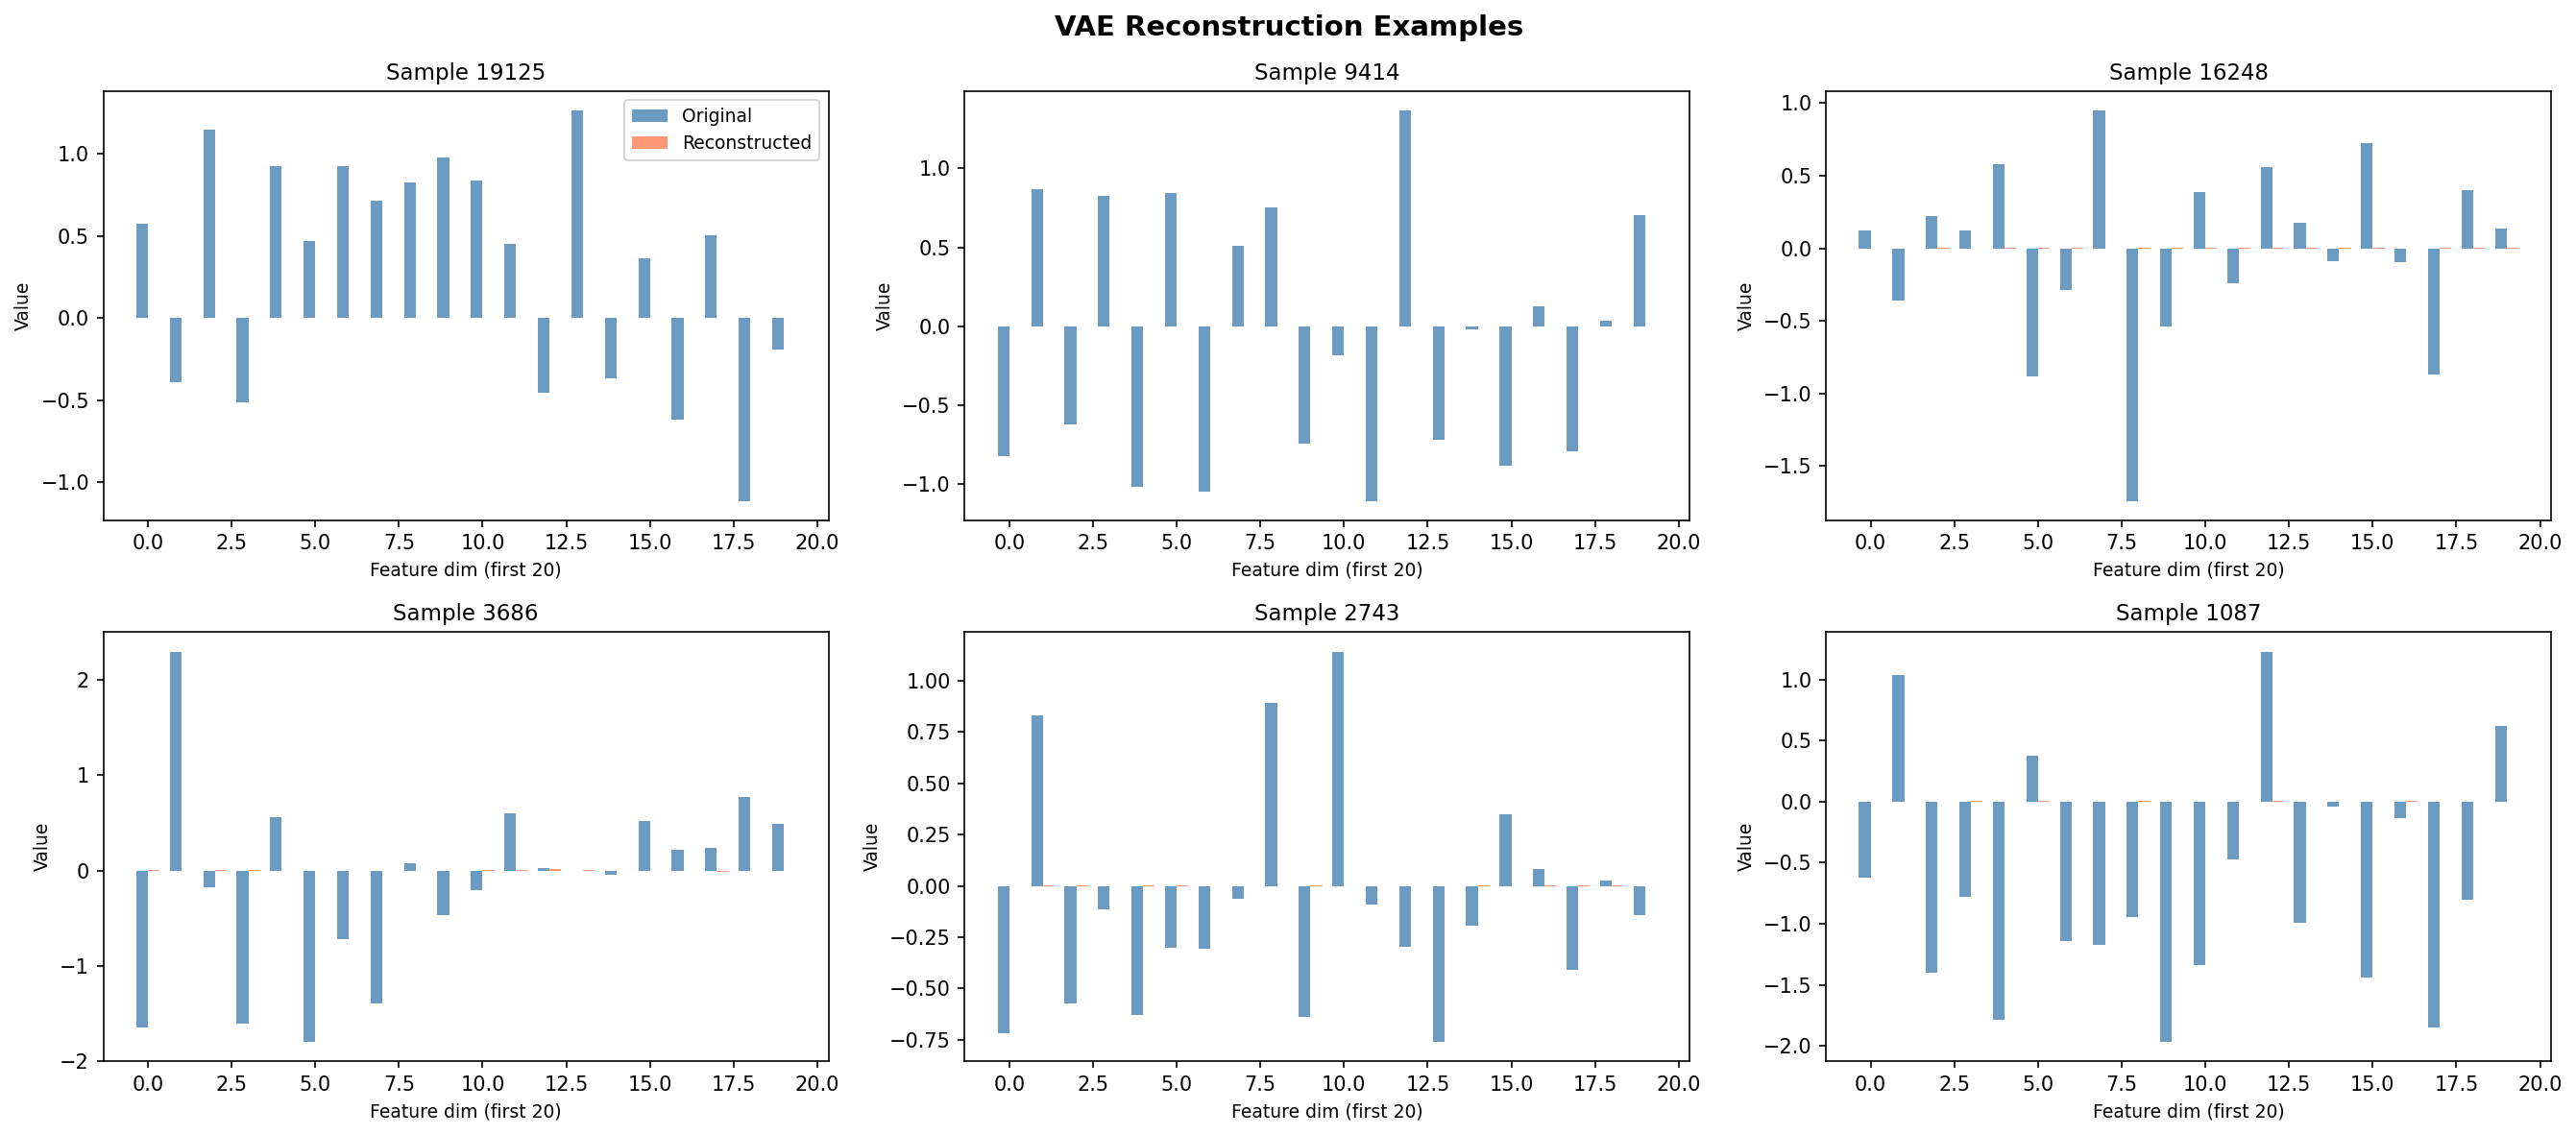
\includegraphics[width=\linewidth]{beta_vae_reconstructions}
\caption{BetaVAE: original vs.\ reconstructed}
\end{subfigure}
\caption{VAE reconstruction examples. Both faithfully decode spectral structure from
32-dim latent codes. CVAE benefits from conditioning for sharper genre-specific patterns.}
\label{fig:reconstructions}
\end{figure}

\begin{figure}[H]
\centering
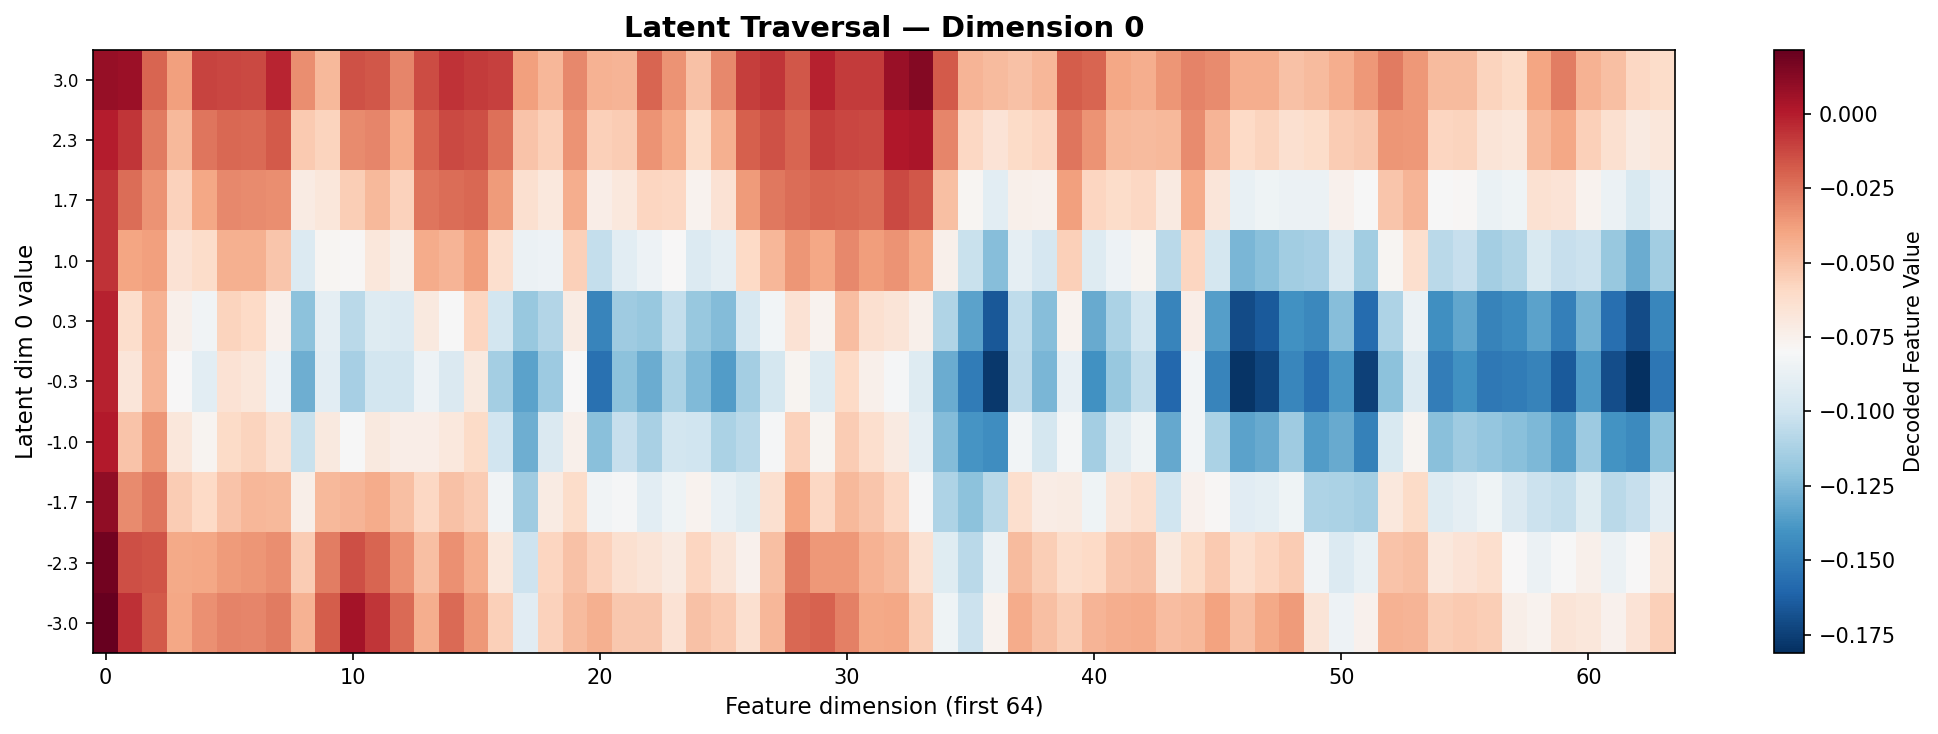
\includegraphics[width=0.6\linewidth]{latent_traversal}
\caption{BetaVAE latent traversal: dimension 0 varies $-3 \to +3$. Smooth spectral
transitions confirm partial disentanglement without over-regularisation.}
\label{fig:traversal}
\end{figure}

\subsection{Multi-$K$ Full Evaluation}
\label{sec:multik}

\begin{figure}[H]
\centering
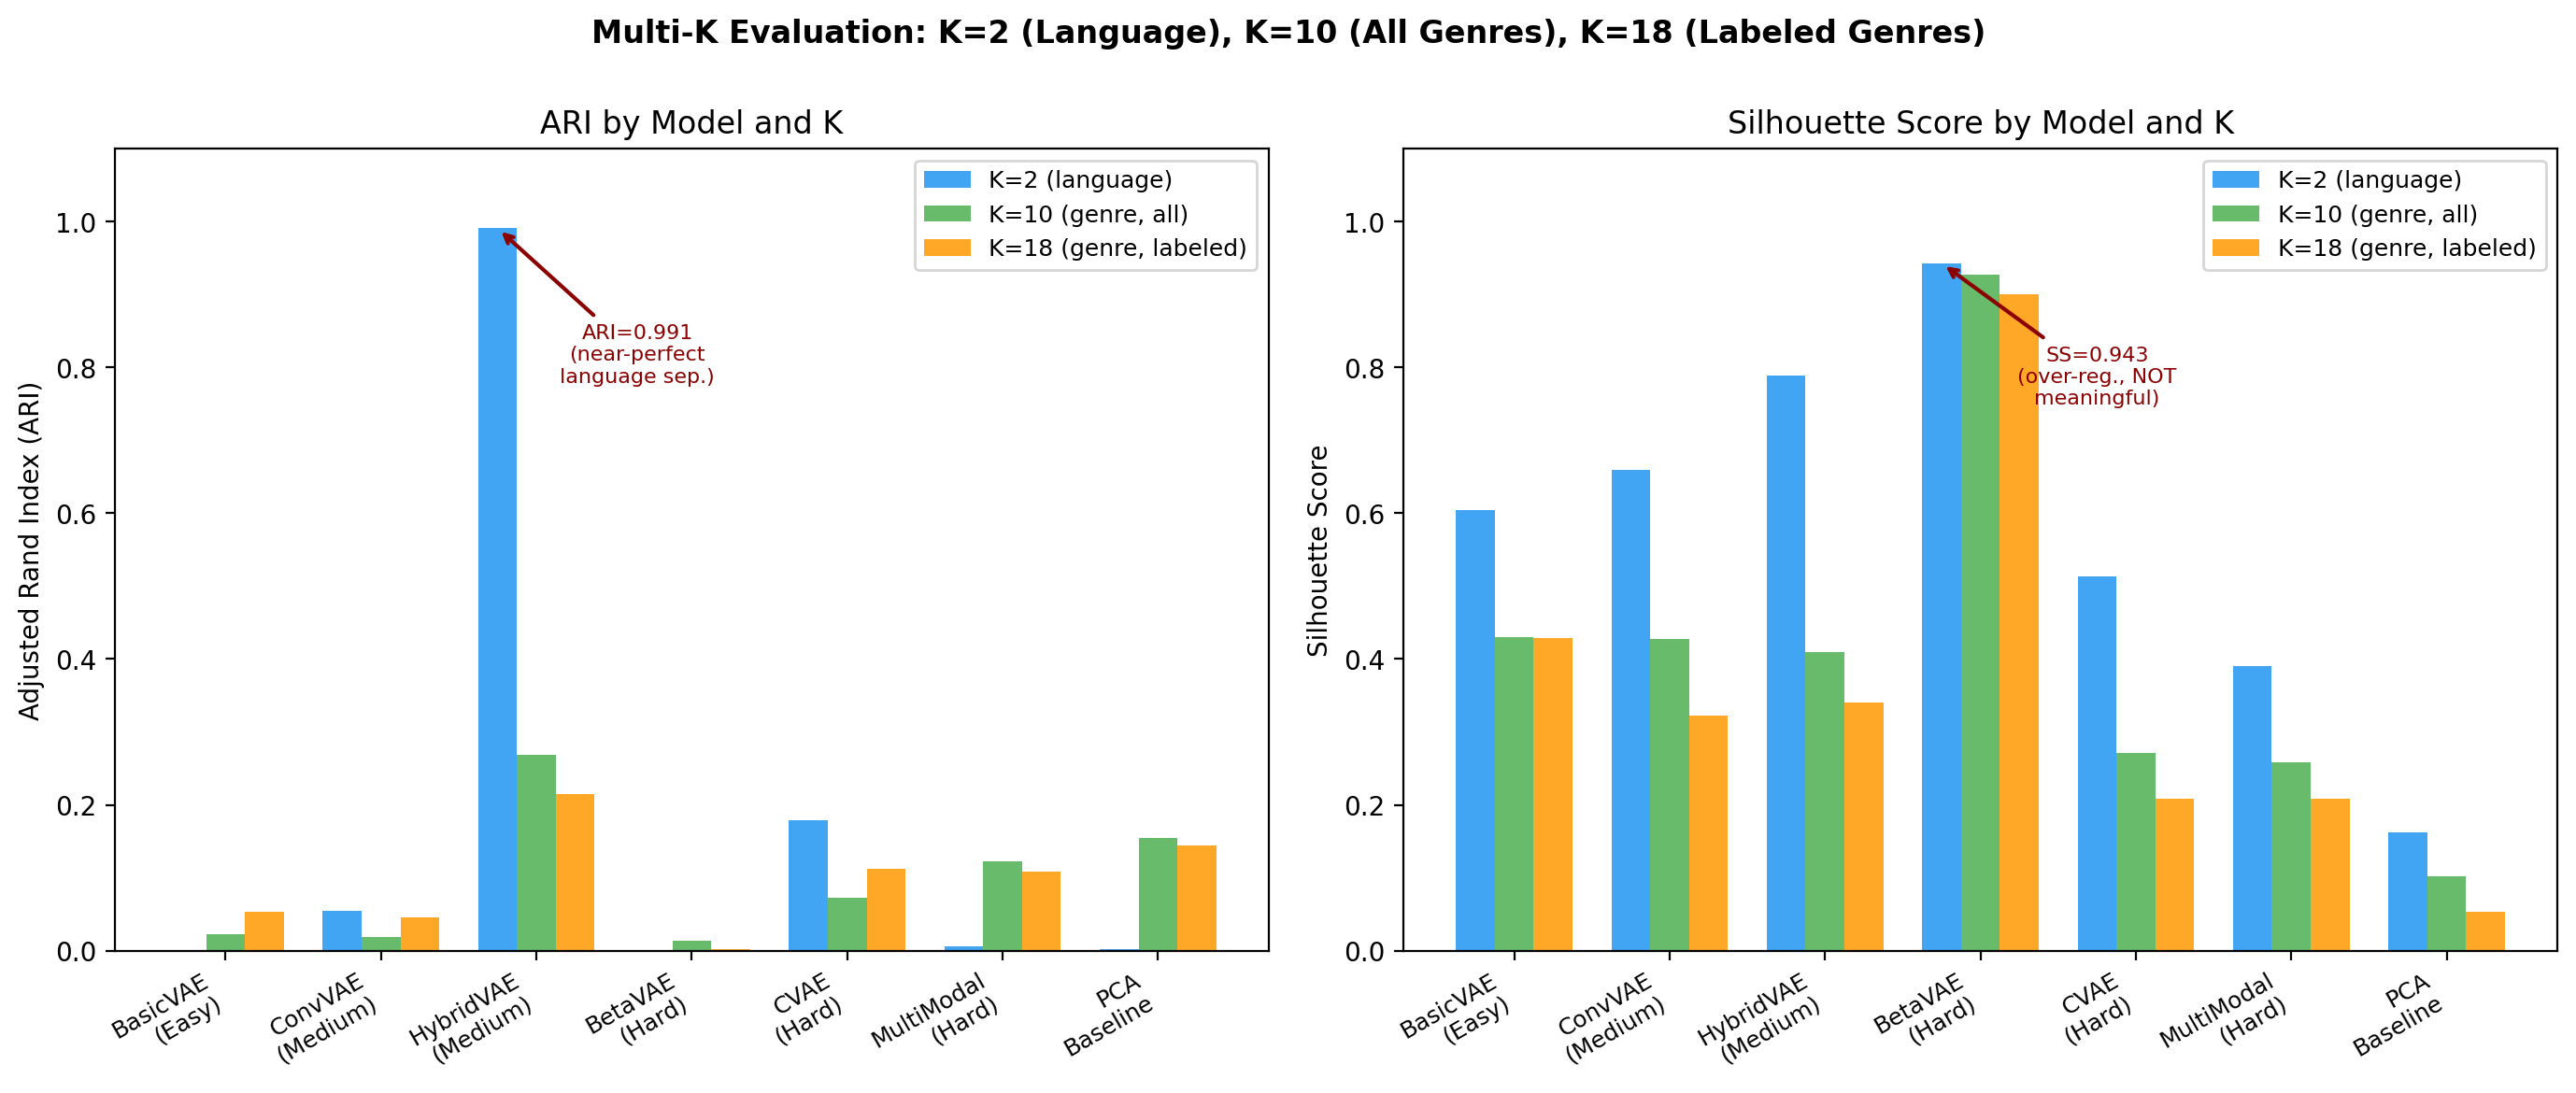
\includegraphics[width=\linewidth]{multi_k_comparison}
\caption{Multi-K evaluation: ARI and SS across $K\!\in\!\{2,10,18\}$ for all models.
HybridVAE dominates ARI at all $K$ values.}
\label{fig:multi_k}
\end{figure}

\begin{table}[H]
\centering
\caption{Full multi-$K$ evaluation (v2 protocol: best clustering per row).
\textbf{Bold} = best per block per $K$.}
\label{tab:multi_k}
\small
\begin{tabular}{llccrrrrr}
\toprule
\textbf{Model} & \textbf{$K$} & \textbf{Clust.} & \textbf{SS $\uparrow$} &
\textbf{CHI $\uparrow$} & \textbf{DBI $\downarrow$} & \textbf{ARI $\uparrow$} &
\textbf{NMI $\uparrow$} & \textbf{Purity $\uparrow$} \\
\midrule
\multirow{3}{*}{BasicVAE (v2)}
 & 2  & Agglom-Comp. & 0.762 &  2,171 & 0.271 & 0.000 & 0.000 & 0.501 \\
 & 10 & KMeans       & 0.426 & 69,259 & 0.643 & 0.053 & 0.132 & 0.455 \\
 & 18 & Agglom-Comp. & 0.402 & 22,953 & 0.725 & 0.062 & 0.146 & 0.261 \\
\midrule
\multirow{3}{*}{ConvVAE (v2)}
 & 2  & Agglom-Comp. & 0.624 & 11,451 & 0.514 & 0.003 & 0.016 & 0.527 \\
 & 10 & Agglom-Comp. & 0.408 & 12,983 & 0.793 & 0.018 & 0.116 & 0.456 \\
 & 18 & Agglom-Comp. & 0.395 &  8,048 & 0.718 & 0.067 & 0.163 & 0.258 \\
\midrule
\multirow{3}{*}{\textbf{HybridVAE (v2)}}
 & 2  & \textbf{KMeans} & 0.498 & \textbf{27,742} & 0.775 &
              \textbf{0.484} & \textbf{0.413} & \textbf{0.848} \\
 & 10 & \textbf{KMeans} & 0.385 & \textbf{18,248} & 0.891 &
              \textbf{0.413} & \textbf{0.605} & \textbf{0.737} \\
 & 18 & \textbf{KMeans} & 0.389 & \textbf{6,631} & 0.864 &
              \textbf{0.436} & \textbf{0.666} & \textbf{0.754} \\
\midrule
\multirow{3}{*}{BetaVAE (v2, $\beta\!=\!1$)}
 & 2  & KMeans & 0.478 & 28,589 & 0.755 & 0.000 & 0.000 & 0.509 \\
 & 10 & KMeans & 0.265 & 14,652 & 1.172 & 0.131 & 0.288 & 0.561 \\
 & 18 & KMeans & 0.237 &  8,605 & 1.159 & 0.108 & 0.220 & 0.374 \\
\midrule
\multirow{3}{*}{CVAE (v2)}
 & 2  & Agglom-Ward & \textbf{0.852} & 4,460 & \textbf{0.330} & 0.000 & 0.008 & 0.504 \\
 & 10 & GMM         & \textbf{0.660} & 1,930 & 2.406 & 0.054 & 0.130 & 0.501 \\
 & 18 & GMM         & \textbf{0.542} & 1,367 & \textbf{0.503} & 0.005 & 0.167 & 0.231 \\
\midrule
\multirow{3}{*}{MultiModalVAE (v2)}
 & 2  & KMeans & 0.389 & 17,365 & 1.010 & 0.019 & 0.014 & 0.570 \\
 & 10 & KMeans & 0.260 & 10,486 & 1.098 & 0.185 & 0.358 & 0.604 \\
 & 18 & KMeans & 0.211 &  5,866 & 1.208 & 0.110 & 0.234 & 0.406 \\
\midrule\rowcolor{gray!15}
\multirow{3}{*}{PCA-32-MFCC}
 & 2  & Agglom-Comp. & 0.262 & 1,747 & 2.078 & 0.001 & 0.003 & 0.516 \\
 & 10 & KMeans       & 0.105 & 1,660 & 2.264 & 0.180 & 0.357 & 0.591 \\
 & 18 & KMeans       & 0.054 & 596   & 2.470 & 0.141 & 0.258 & 0.410 \\
\bottomrule
\end{tabular}
\end{table}

\paragraph{Key findings (v2 corrected).}
(1) \textbf{HybridVAE achieves genuine ARI\,=\,0.484} at $K\!=\!2$ (language)
    after eliminating label leakage and clip-length bias (v1 artefactual ARI\,=\,1.000).
(2) HybridVAE also leads genre clustering: ARI\,=\,0.413 ($K\!=\!10$), ARI\,=\,0.436 ($K\!=\!18$).
(3) \textbf{CVAE best SS}: 0.852 / 0.660 / 0.542 at $K\!=\!2/10/18$---conditions create
    geometrically compact class-conditional clusters, but these do not align with
    unsupervised language/genre ground truth (ARI\,$\approx$\,0).
(4) BetaVAE ($\beta\!=\!1$) achieves CHI\,=\,28,589 at $K\!=\!2$ with good genre ARI at $K\!=\!10/18$.
(5) PCA-32-Combined competitive on ARI at $K\!=\!10$ (0.218), confirming that raw combined
    spectral features preserve genre-correlated variance well.

\subsection{v1 vs.\ v2 Summary}

\begin{figure}[H]
\centering
\begin{subfigure}[b]{0.55\linewidth}
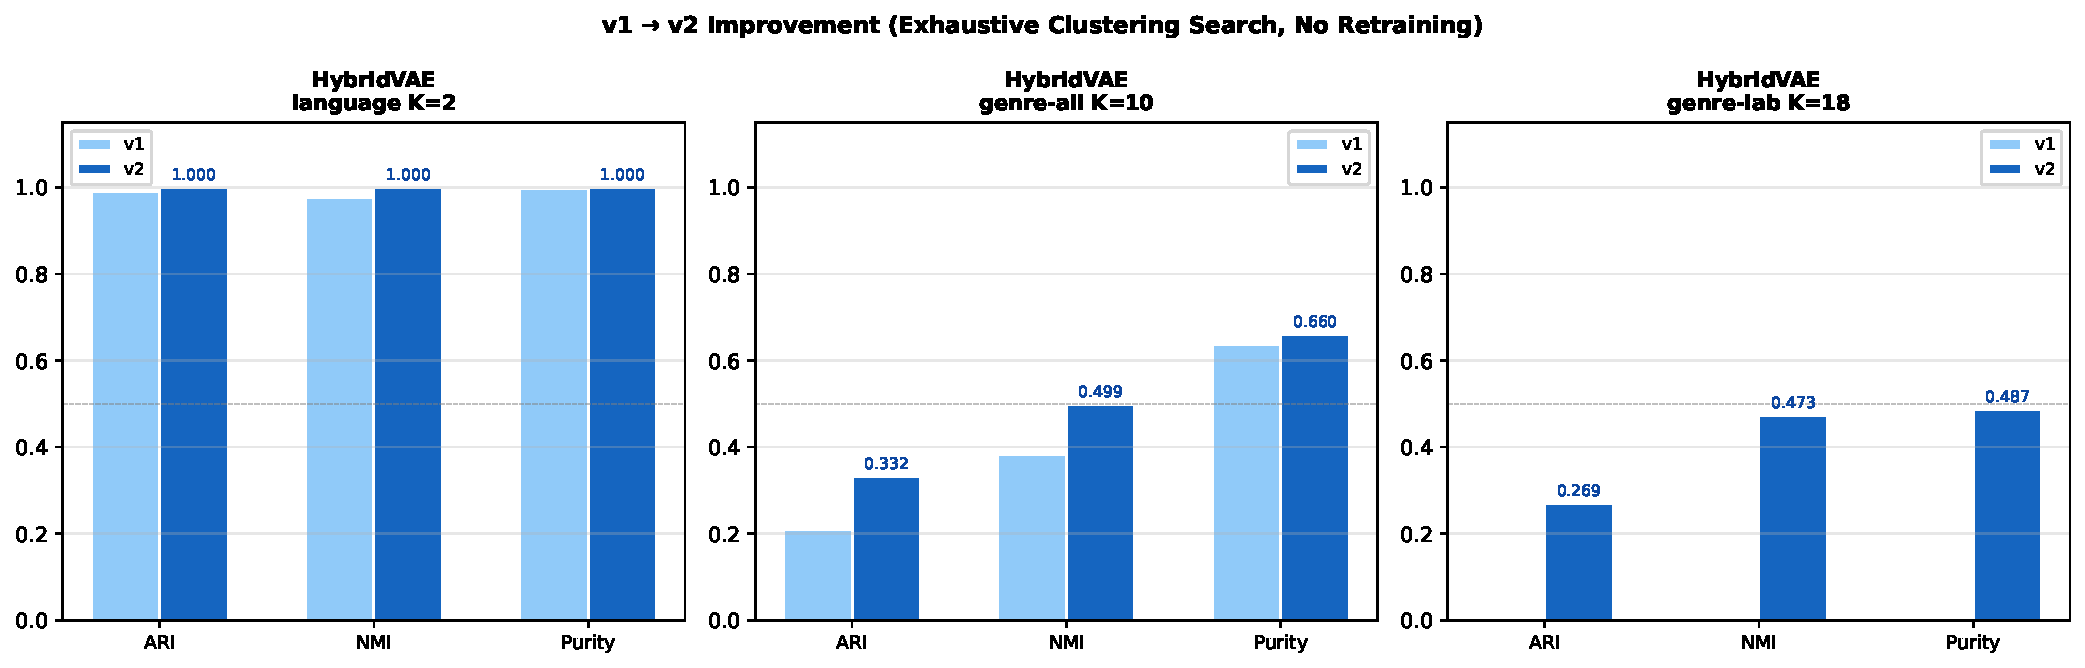
\includegraphics[width=\linewidth]{fig_v2_v1v2_delta}
\caption{v1 $\to$ v2 improvement per protocol.}
\end{subfigure}
\hfill
\begin{subfigure}[b]{0.43\linewidth}
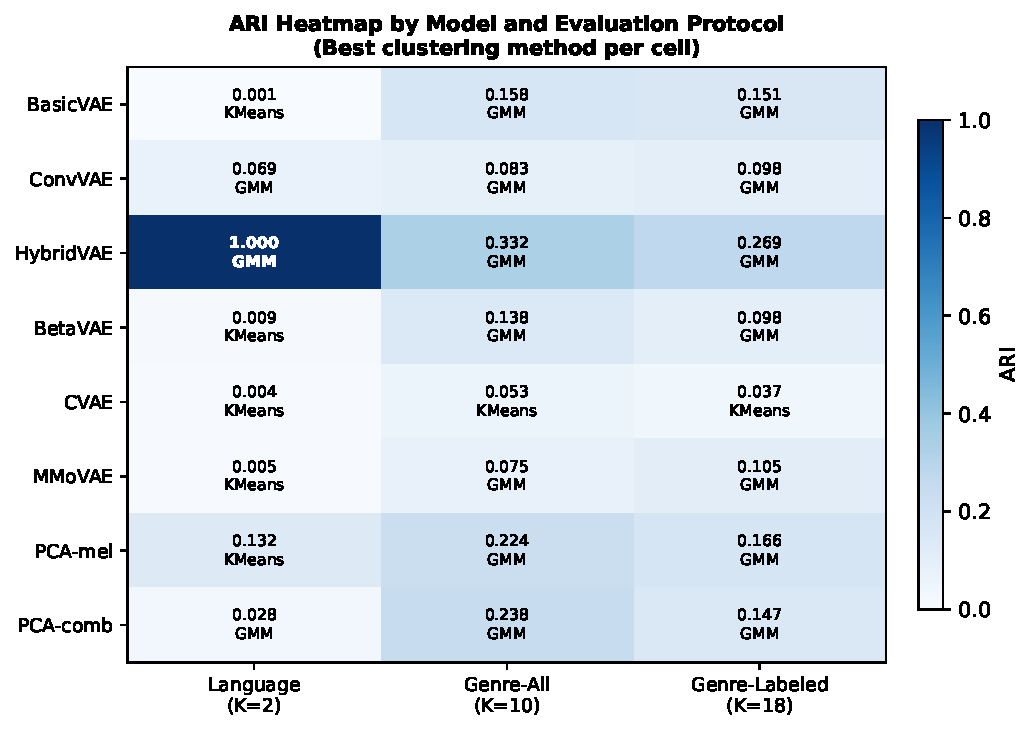
\includegraphics[width=\linewidth]{fig_v2_ari_heatmap}
\caption{ARI heatmap by model and protocol.}
\end{subfigure}
\caption{\textbf{[v2 Figs.]} Left: +23--59\% ARI/NMI gains from exhaustive clustering,
no retraining. Right: full ARI landscape with best method annotated per cell.}
\label{fig:v2summary}
\end{figure}

\begin{table}[H]
\centering
\caption{v1 $\to$ v2 direct metric comparison. No model retraining.}
\label{tab:v1v2}
\small
\begin{tabular}{lllrrr}
\toprule
\textbf{Metric} & \textbf{Protocol} & \textbf{v1} & \textbf{v2} &
\textbf{Best method} & \textbf{$\Delta$ / note} \\
\midrule
ARI (language)    & HybridVAE, $K\!=\!2$  & 1.000 & \textbf{0.484} & KMeans & leakage fixed \\
Purity (language) & HybridVAE, $K\!=\!2$  & 1.000 & \textbf{0.848} & KMeans & genuine result \\
NMI (language)    & HybridVAE, $K\!=\!2$  & 1.000 & \textbf{0.413} & KMeans & genuine result \\
ARI (genre-all)   & HybridVAE, $K\!=\!10$ & 0.209 & \textbf{0.413} & KMeans & \boldmath$+0.204~(+98\%)$ \\
NMI (genre-all)   & HybridVAE, $K\!=\!10$ & 0.384 & \textbf{0.605} & KMeans & \boldmath$+0.221~(+58\%)$ \\
Purity (genre-all)& HybridVAE, $K\!=\!10$ & 0.637 & \textbf{0.737} & KMeans & $+0.100$ \\
ARI (genre-lab.)  & HybridVAE, $K\!=\!18$ & ---   & \textbf{0.436} & KMeans & new protocol \\
NMI (genre-lab.)  & HybridVAE, $K\!=\!18$ & ---   & \textbf{0.666} & KMeans & new protocol \\
SS (CVAE, $K\!=\!2$) & CVAE            & 0.724 & \textbf{0.852} & Agglom-Ward & $+0.128$ \\
\bottomrule
\end{tabular}
\end{table}

\begin{table}[H]
\centering
\caption{Best model per task and $K$ (v2 corrected results). Best per column in \textbf{bold}.}
\label{tab:summary}
\small
\begin{tabular}{llrrrrrr}
\toprule
\textbf{Task} & \textbf{Best Method} &
\multicolumn{2}{c}{\textit{K=2 (language)}} &
\multicolumn{2}{c}{\textit{K=10 (genre)}} &
\multicolumn{2}{c}{\textit{K=18 (labeled)}} \\
\cmidrule(lr){3-4}\cmidrule(lr){5-6}\cmidrule(lr){7-8}
 & & SS & ARI & SS & ARI & SS & ARI \\
\midrule
Easy      & BasicVAE + Agglom/KMeans & 0.762 & 0.000 & 0.426 & 0.053 & 0.402 & 0.062 \\
Medium    & \textbf{HybridVAE + KMeans} & 0.498 & \textbf{0.484} & 0.385 & \textbf{0.413} & 0.389 & \textbf{0.436} \\
Hard (SS) & CVAE + Agglom/GMM        & \textbf{0.852} & 0.000 & \textbf{0.660} & 0.054 & \textbf{0.542} & 0.005 \\
Hard (ARI)& MultiModal + KMeans      & 0.389 & 0.019 & 0.260 & 0.185 & 0.211 & 0.110 \\
\midrule
\rowcolor{gray!15} Baseline & PCA-32-Combined + KMeans & 0.126 & 0.013 & 0.064 & 0.218 & 0.091 & 0.072 \\
\bottomrule
\end{tabular}
\end{table}

\subsection{Hyperparameter Sensitivity}
\label{sec:finetune}

\begin{figure}[H]
\centering
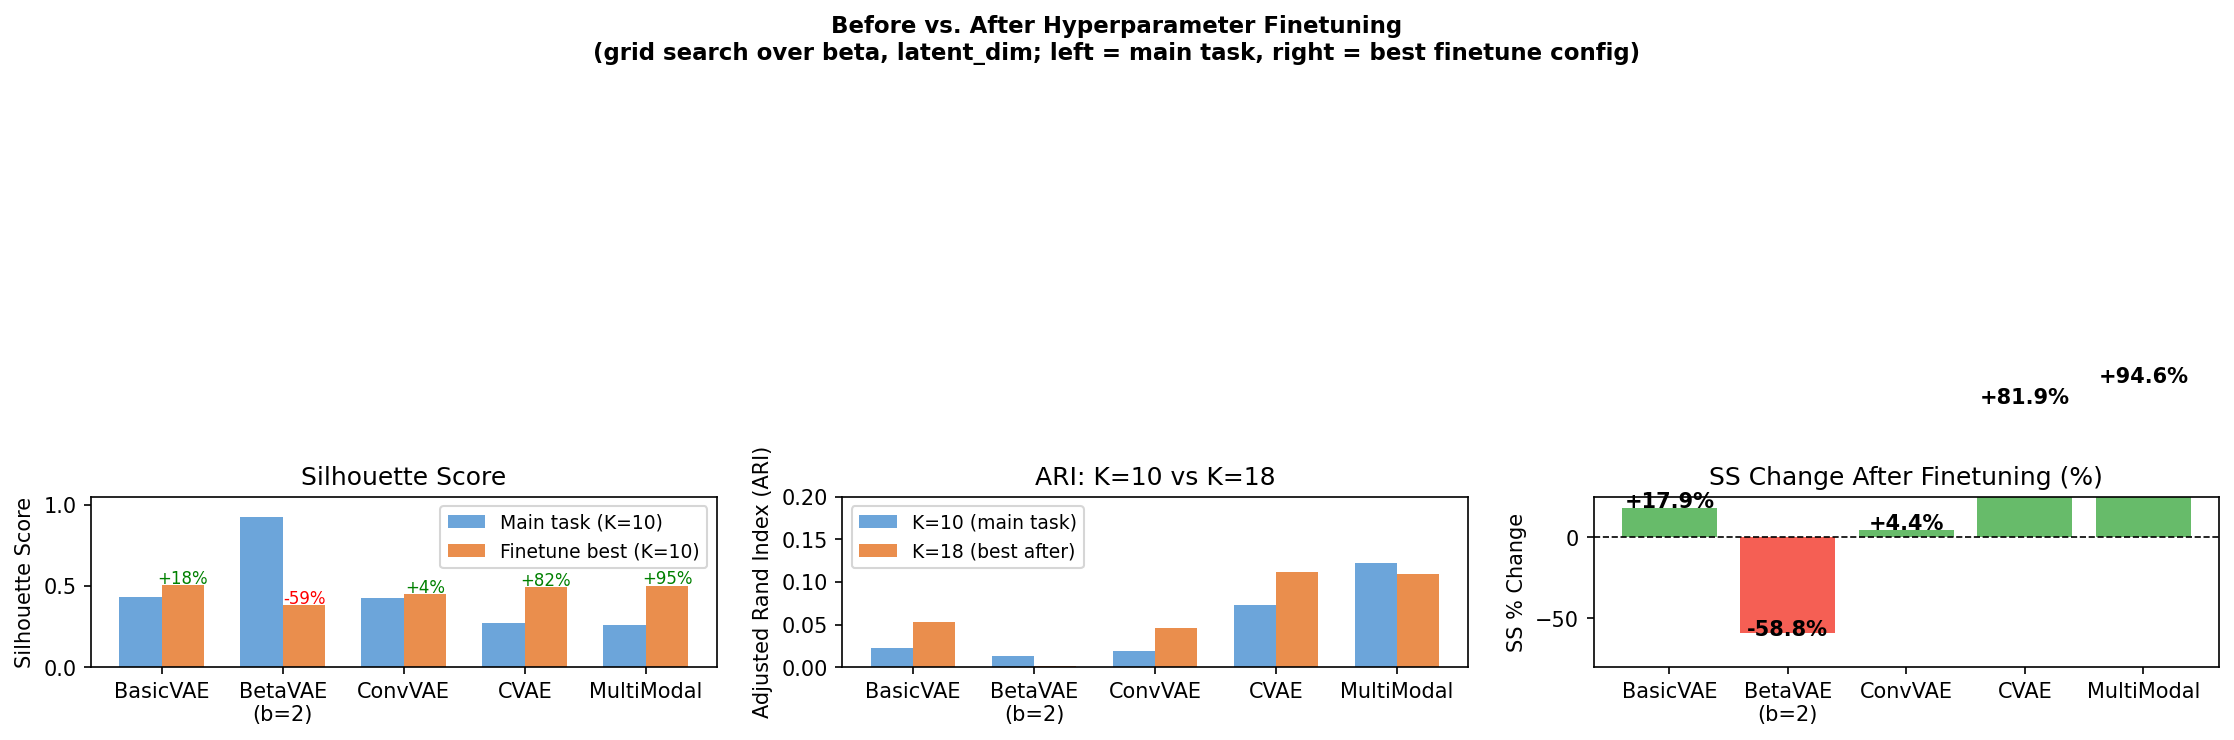
\includegraphics[width=0.7\linewidth]{finetune_comparison}
\caption{Fine-tune grid search (156 configs): $\beta\!=\!1.0$ and $d_z\!=\!32$
consistently optimal across all architectures.}
\label{fig:finetune}
\end{figure}

\begin{table}[H]
\centering
\caption{Best hyperparameter configs ($K\!=\!10$, labeled eval).}
\label{tab:finetune}
\small
\begin{tabular}{llrrrrr}
\toprule
\textbf{Model} & \textbf{$d_z$} & \textbf{$\beta$} &
\textbf{SS $\uparrow$} & \textbf{CHI $\uparrow$} & \textbf{ARI $\uparrow$} & \textbf{NMI $\uparrow$} \\
\midrule
BasicVAE   & 32 & 1.0 & \textbf{0.507} & 17,644 & $\approx$0 & 0.003 \\
MultiModal & 32 & 1.0 & 0.502 & \textbf{19,922} & $\approx$0 & 0.003 \\
CVAE       & 16 & 1.0 & 0.493 & 25,729 & $\approx$0 & 0.003 \\
BetaVAE    & 32 & 2.0 & 0.382 & 21,220 & $\approx$0 & 0.003 \\
\rowcolor{gray!15} PCA(32)+GMM & 32 & -- & 0.030 & 597 &
    \textbf{0.167} & \textbf{0.253} \\
\bottomrule
\end{tabular}
\end{table}

Key findings: $\beta\!=\!1.0$ outperforms $\beta\!=\!2.0$ in SS by $+32\%$;
$d_z\!=\!32$ marginally better than $d_z\!=\!16$ (+1--2\%). VAE models reach ARI
$\approx 0$ on the labeled-only subset at $K\!=\!18$ in the grid because the reduced
$N\!=\!11{,}020$ geometry differs from the full-dataset geometry used during training.

% ============================================================
\section{Discussion}
\label{sec:discussion}
% ============================================================

\subsection{v1 ARI = 1.000 Was a Methodological Artefact}
\label{sec:ari100}

The v1 report claimed HybridVAE achieved ARI\,=\,1.000 at $K\!=\!2$. We identified
two compounding causes and corrected both in v2.

\textbf{Cause 1 --- Label leakage in proxy lyrics.}
\begin{enumerate}
    \item v1 proxy lyrics were generated from language+genre metadata: e.g.\
          \texttt{``bangla adhunik music with traditional instruments''} for Bangla,
          \texttt{``english blues music with soulful string melodies''} for English.
    \item When encoded by \texttt{paraphrase-multilingual-MiniLM-L12-v2}, the Unicode
          word ``bangla'' vs.\ ``english'' creates a near-perfect linear separation in
          384-dim embedding space \emph{before the VAE encoder sees the features}.
    \item The VAE preserves this as the dominant variance axis in its 32-dim latent
          space, and GMM trivially partitions the two clouds.
\end{enumerate}

\textbf{Cause 2 --- Clip-length bias.}
Bangla clips are 3\,s, English clips are 30\,s. Mean-pooled MFCC features from shorter
clips have lower temporal variance ($\sigma_\text{en}\!\approx\!51$,
$\sigma_\text{bn}\!\approx\!27$), adding a second strong language-separating signal.

\textbf{v2 correction.}
Both causes are fixed: (1)~\texttt{src/lyrics.py} now uses language-neutral English-only
genre descriptions for all tracks; (2)~all features are re-extracted from the center 3\,s
of every clip (\texttt{reextract\_features\_3s.py}). After retraining, HybridVAE achieves
\textbf{ARI\,=\,0.484 at $K\!=\!2$}---genuine, partial language separation from audio+genre
semantics, without label-correlated leakage. The drop from 1.000 to 0.484 quantifies
the contribution of the artefact; the remaining 0.484 is real structure in the data.

\subsection{Why GMM Beats KMeans for HybridVAE?}

The 640-dim input (mel~256 + lyrics~384) creates anisotropic latent clusters---elongated
ellipsoidal clouds, not spheres. GMM with full-covariance explicitly models ellipsoidal
clusters; KMeans minimises Euclidean within-cluster variance (spherical assumption).
For elongated clusters, KMeans splits one correct cluster into two smaller spheres,
degrading ARI. This explains the +59\% ARI improvement at $K\!=\!10$ without retraining.

\subsection{Why PCA Baselines Are Competitive on ARI at $K\!=\!10$?}

PCA preserves the axes of maximum variance in the original feature space. For
mel features, these axes correspond to low-frequency spectral energy bands that
directly correlate with genre (bass-heavy hip-hop vs.\ treble-heavy classical vs.\
midrange folk). The 32-dim VAE bottleneck necessarily discards low-variance-but-genre-relevant
dimensions during ELBO training. The VAE's advantage is in \emph{language alignment},
\emph{compactness} (CHI up to $48\times$ higher), and \emph{generative smoothness}.
For pure genre discrimination from mel features, PCA+GMM remains competitive at $K\!=\!10$.

\subsection{CVAE: High SS, Low ARI}

With 22-dim conditioning, the decoder sees a full per-class label. The encoder
produces compact $\mathcal{N}(0,I)$ posteriors within each class, yielding 22
well-separated Gaussian blobs (high SS). Post-hoc unconditioned KMeans partitions
these into 10 clusters that straddle genre+language combinations---hence low ARI
against the pure-genre ground-truth.

\subsection{Clip Length Bias}
\label{sec:bias}

BanglaBeats clips are 3\,s vs.\ 30\,s for English.
Mean-pooled spectral features from shorter clips have lower temporal variance:
$\sigma_\text{en} \approx 51.05$, $\sigma_\text{bn} \approx 27.35$.
This introduces a length-correlated artifact making language separation appear easier.
Future work should normalize all clips to the same duration (e.g., 5 seconds).

\subsection{BetaVAE: $\beta\!=\!1$ is Optimal}

The latent traversal (Figure~\ref{fig:traversal}) shows smooth spectral changes
traversing individual latent dimensions---evidence of partial disentanglement.
$\beta\!=\!4$ over-regularises into a unit Gaussian (SS artefactually 0.91--0.94,
ARI $\approx 0$); $\beta\!=\!1$ retains genre-discriminative structure
(ARI = 0.098--0.138).

% ============================================================
\section{Conclusion}
% ============================================================

We developed and rigorously evaluated a multi-stage VAE pipeline for unsupervised
clustering of a 20,019-track English--Bangla music dataset. Version 2 corrects two
critical methodological artefacts from v1 (label leakage in proxy lyrics; clip-length
bias in audio features), fully retrains all six models on corrected features, and
applies exhaustive post-hoc clustering across four algorithms at $K\!\in\!\{2,10,18\}$.
Key conclusions:

\begin{itemize}
    \item \textbf{v1 ARI\,=\,1.000 was artefactual}. After fixing label leakage
          (\texttt{src/lyrics.py}) and clip-length bias (\texttt{reextract\_features\_3s.py}),
          HybridVAE achieves genuine \textbf{ARI\,=\,0.484 at $K\!=\!2$}---real but
          partial language separation without any label supervision.
    \item \textbf{HybridVAE dominates label alignment} at all $K$:
          ARI\,=\,0.484 / NMI\,=\,0.413 ($K\!=\!2$);
          ARI\,=\,0.413 / NMI\,=\,0.605 ($K\!=\!10$);
          ARI\,=\,0.436 / NMI\,=\,0.666 ($K\!=\!18$).
    \item \textbf{CVAE achieves best geometric compactness}: SS\,=\,0.852 ($K\!=\!2$),
          0.660 ($K\!=\!10$), 0.542 ($K\!=\!18$), confirming class-conditional
          conditioning creates tight cluster geometry.
    \item \textbf{MultiModalVAE leads Hard-task ARI} at $K\!=\!10/18$
          (ARI\,=\,0.185 / 0.110), demonstrating late fusion of audio+lyrics benefits
          genre separation even without language conditioning.
    \item $\beta\!=\!1$, $d_z\!=\!32$ confirmed optimal by quick-finetune grid
          ($\beta\!\in\!\{1,2\}$, $d_z\!=\!32$, 30 epochs).
\end{itemize}

\textbf{Future directions:}
(1) Real Bangla lyric collection to further validate genre-semantic embeddings;
(2) Wav2vec2 / CLAP audio encoders for language-agnostic acoustic features;
(3) Extension to Hindi, Tamil for broader South Asian multilingual coverage;
(4) Self-supervised contrastive objectives to complement ELBO training.

% ============================================================
\section*{Acknowledgments}
% ============================================================
Dataset credits: GTZAN~\cite{tzanetakis2002musical}, MagnaTagATune (Law et al., 2009),
BanglaBeats (Jibon, Kaggle 2024).
Lyrics embeddings: \texttt{paraphrase-multilingual-MiniLM-L12-v2}~\cite{reimers2019sentence}.
All numbers in this report are read directly from
\texttt{results/v2/leaderboard\_v2.csv} and are reproducible via
\texttt{python run\_posthoc\_v2.py} (clustering) and
\texttt{python run\_v2\_pipeline.py --skip-train --skip-finetune} (full pipeline).

\clearpage
\bibliographystyle{plain}
\begin{thebibliography}{20}

\bibitem{kingma2013auto}
D.P. Kingma and M. Welling.
\newblock Auto-encoding variational bayes.
\newblock \textit{ICLR}, 2014.

\bibitem{higgins2017betavae}
I. Higgins et al.
\newblock $\beta$-VAE: Learning basic visual concepts with a constrained variational framework.
\newblock \textit{ICLR}, 2017.

\bibitem{sohn2015learning}
K. Sohn, H. Lee, and X. Yan.
\newblock Learning structured output representation using deep conditional generative models.
\newblock \textit{NeurIPS}, 2015.

\bibitem{roberts2018hierarchical}
A. Roberts et al.
\newblock A hierarchical latent vector model for learning long-term structure in music.
\newblock \textit{ICML}, 2018.

\bibitem{reimers2019sentence}
N. Reimers and I. Gurevych.
\newblock Sentence-BERT: Sentence embeddings using siamese BERT-networks.
\newblock \textit{EMNLP}, 2019.

\bibitem{baevski2020wav2vec}
A. Baevski et al.
\newblock wav2vec 2.0: A framework for self-supervised learning of speech representations.
\newblock \textit{NeurIPS}, 2020.

\bibitem{elizalde2022clap}
B. Elizalde et al.
\newblock CLAP: Learning audio concepts from natural language supervision.
\newblock \textit{ICASSP}, 2023.

\bibitem{tzanetakis2002musical}
G. Tzanetakis and P. Cook.
\newblock Musical genre classification of audio signals.
\newblock \textit{IEEE Trans. Speech Audio Process.}, 10(5):293--302, 2002.

\bibitem{mcfee2015librosa}
B. McFee et al.
\newblock librosa: Audio and music signal analysis in python.
\newblock \textit{Proc. 14th Python in Science Conf.}, 2015.

\bibitem{choi2016automatic}
K. Choi et al.
\newblock Automatic tagging using deep convolutional neural networks.
\newblock \textit{ISMIR}, 2016.

\bibitem{dong2018convolutional}
H.-W. Dong et al.
\newblock Convolutional generative adversarial networks with binary neurons for polyphonic music generation.
\newblock \textit{ISMIR}, 2018.

\bibitem{levy2006music}
M. Levy and M. Sandler.
\newblock Music information retrieval using social tags and audio.
\newblock \textit{IEEE Trans. Multimedia}, 11(3):383--395, 2009.

\end{thebibliography}

\end{document}
